%\documentclass[aps,prb,twocolumn,superscriptaddress,footinbib,amsmath,amssymb,floatfix]{revtex4}
\documentclass[aps,prb,onecolumn,preprint,superscriptaddress,footinbib,amsmath,amssymb,floatfix]{revtex4}
\usepackage[dvips]{epsfig}
\usepackage{graphicx}
\usepackage{ifthen}
\usepackage{dcolumn}% Align table columns on decimal point
\usepackage{bm}% bold math
\usepackage{multirow}
\usepackage{booktabs}
\usepackage{bm}% bold math
\usepackage{amsbsy}
\usepackage{amsmath}
\usepackage{amssymb}
\usepackage{subfigure}
%\usepackage{wrapfig}

%Definition of new commands
\newcommand{\f}[2]{\ensuremath{\frac{\displaystyle{#1}}{\displaystyle{#2}}}}
\newcommand{\lr}[1]{\langle{#1}\rangle}
\newcommand{\colv}[2] {\left(\begin{array}{c} #1 \\ #2 \end{array}\right)}
\renewcommand{\thefootnote}{\fnsymbol{footnote}}
\newcommand{\be} {\begin{eqnarray}}
\newcommand{\ee} {\end{eqnarray}}
%--------------------------------------------------------------------------
%EQ COMMANDS
%--------------------------------------------------------------------------
\newcommand{\two}{\mspace{-2.0mu}}
\newcommand{\four}{\mspace{-4.0mu}}
\newcommand{\plus}{\mspace{-4.5mu}+\mspace{-3.5mu}}
\newcommand{\minus}{\mspace{-4.5mu}-\mspace{-3.5mu}}
\newcommand{\pp}{'\mspace{-2.0mu}'}
\newcommand{\xlb}[4]{#1\ifthenelse{\equal{#2}{0}}{}{_{\alpha #2}}
\mspace{-2.0mu}\genfrac{(}{)}{0pt}{1}{\ifthenelse{\equal{#3}{0}}{0}{l #3}} 
{\ifthenelse{\equal{#4}{0}}{0}{b #4}}}

\newcommand{\xkv}[4]{#1\mspace{-5.0mu}\left(\mspace{-8.0mu}
\begin{smallmatrix}#2\four{}\four{}\mspace{-8.0mu}&\pmb{\kappa}#3\\&\nu 
#4\end{smallmatrix}\mspace{-5.0mu}\right)}

\newcommand{\evect}[6]{#1\mspace{-4.0mu}\left(\mspace{-8.0mu}
\begin{smallmatrix}#2\mspace{-8.0mu}&\pmb{\kappa} #3 &b #5\\&\nu #4 &
\alpha #6\end{smallmatrix}\mspace{-5.0mu}\right)}

\newcommand{\varmat}[8]{\mspace{-5.0mu}\left(\mspace{-8.0mu}
\begin{smallmatrix}\ifthenelse{\equal{#3}{0}}{\mspace{-8.0mu}&b_{#1}&b_{#2}
\\&\alpha_{#1}&\alpha_{#2}} {\ifthenelse{\equal{#7}{0}}{#1\mspace{-8.0mu}&
\pmb{\kappa}#2#3\mspace{-8.0mu}&\pmb{\kappa}#4#5\mspace{-8.0mu}&\pmb{\kappa}
#6\\&\nu#2&\nu#4&\nu#6} {#1\mspace{-8.0mu}&\pmb{\kappa}#2#3\mspace{-8.0mu}&
\pmb{\kappa}#4#5\mspace{-8.0mu}&\pmb{\kappa}#6#7\mspace{-8.0mu}&\pmb{\kappa}
#8\\&\nu#2&\nu#4&\nu#6&\nu#8}}\end{smallmatrix}\mspace{-5.0mu}\right)}

\newcommand{\EXP}[1]{\exp\mspace{-5.0mu}\left[#1\right]\mspace{-3.0mu}}

\newcommand{\tpp}[2]{\left(\mspace{-2.0mu}\xkv{\omega}{}{}{}#1\xkv{\omega}
{}{'}{'}#2\xkv{\omega}{}{\pp}{\pp}\mspace{-2.0mu}\right)}



%--------------------------------------------------------------------------
\newcommand{\SUM}[2]{\ifthenelse{\equal{#1}{0}}{\sum_{
\alpha_{#2},b_{#2},l_{#2}}^{3,n,N}} {\ifthenelse{\equal{#1}{1}}{\sum_{
\alpha_{#2},b_{#2}}^{3,n}}{\sum_{\pmb{\kappa}#2,\nu#2}^{N,3n}}}}

\newcommand{\SUMprime}[2]{\ifthenelse{\equal{#1}{0}}
{\sum_{\alpha_{#2},b_{#2},l_{#2}}^{3,n,N}} 
{\ifthenelse{\equal{#1}{1}}{\sum_{\alpha_{#2},b_{#2}}^{3,n}}
{\sum_{\pmb{\kappa}^{'}#2,\nu#2}^{N,3n}}}}

\newcommand{\SUMalpha}[2]{\ifthenelse{\equal{#1}{0}}
{\sum_{\alpha_{#2}}^{3}} {\ifthenelse{\equal{#1}{1}}
{\sum_{\alpha_{#2},b_{#2}}^{3,n}}{\sum_{\pmb{\kappa}#2,\nu#2}^{N,3n}}}}
%--------------------------------------------------------------------------
\newcommand{\SUMalphap}[2]{\ifthenelse{\equal{#1}{0}}
{\sum_{\alpha'_{#2}}^{3}} {\ifthenelse{\equal{#1}{1}}
{\sum_{\alpha'_{#2},b'_{#2}}^{3,n}}{\sum_{\pmb{\kappa}#2,\nu#2}^{N,3n}}}}

\newcommand{\SUMb}[2]{\ifthenelse{\equal{#1}{0}}{\sum_{b_{#2}}^{n}}
 {\ifthenelse{\equal{#1}{1}}{\sum_{\alpha_{#2},b_{#2}}^{3,n}}
{\sum_{\pmb{\kappa}#2,\nu#2}^{N,3n}}}}

\newcommand{\SUMbp}[2]{\ifthenelse{\equal{#1}{0}}{\sum_{b'_{#2}}^{n}}
 {\ifthenelse{\equal{#1}{1}}{\sum_{\alpha'_{#2},b'_{#2}}^{3,n}}
{\sum_{\pmb{\kappa}#2,\nu#2}^{N,3n}}}}

\newcommand{\SUMl}[2]{\ifthenelse{\equal{#1}{0}}{\sum_{l_{#2}}^{N}}
 {\ifthenelse{\equal{#1}{1}}{\sum_{\alpha_{#2},b_{#2}}^{3,n}}
{\sum_{\pmb{\kappa}#2,\nu#2}^{N,3n}}}}

\newcommand{\SUMlp}[2]{\ifthenelse{\equal{#1}{0}}{\sum_{l'_{#2}}^{N}}
 {\ifthenelse{\equal{#1}{1}}{\sum_{\alpha'_{#2},b'_{#2}}^{3,n}}
{\sum_{\pmb{\kappa}#2,\nu#2}^{N,3n}}}}

\newcommand{\abcdt}[5]{\mspace{-4.0mu}\left(\mspace{-8.0mu}
\begin{smallmatrix}&\ifthenelse{\equal{#1}{}}{a}{#1}&\ifthenelse
{\equal{#3}{}}{c}{#3}\\&\ifthenelse{\equal{#2}{}}{b}{#2}&\ifthenelse
{\equal{#4}{}}{d}{#4}\end{smallmatrix}\mspace{-2.0mu};\ifthenelse
{\equal{#5}{}}{t}{#5}\right)}

\newcommand{\abcd}[4]{\mspace{-4.0mu}\left(\mspace{-8.0mu}
\begin{smallmatrix}&\ifthenelse{\equal{#1}{}}{a}{#1}&\ifthenelse
{\equal{#3}{}}{c}{#3}\\&\ifthenelse{\equal{#2}{}}{b}{#2}&\ifthenelse
{\equal{#4}{}}{d}{#4}\end{smallmatrix}\mspace{-3.0mu}\right)}

\newcommand{\abt}[3]{\mspace{-4.0mu}\left(\mspace{-8.0mu}\begin
{smallmatrix}&\ifthenelse{\equal{#1}{}}{a}{#1} \\&\ifthenelse{
\equal{#2}{}}{b}{#2}\end{smallmatrix}\mspace{-2.0mu};
\ifthenelse{\equal{#3}{}}{t}{#3}\right)}

\newcommand{\ab}[2]{\mspace{-4.0mu}\left(\mspace{-8.0mu}
\begin{smallmatrix}&\ifthenelse{\equal{#1}{}}{a}{#1} \\&\ifthenelse
{\equal{#2}{}}{b}{#2}\end{smallmatrix}\mspace{-3.0mu}\right)}

\newcommand{\kvbat}{\mspace{-4.0mu}\left(\mspace{-8.0mu}
\begin{smallmatrix} &\pmb{\kappa} &b \\ &\nu &\alpha\end{smallmatrix}
\mspace{-2.0mu};t\right)}
%--------------------------------------------------------------------------


\newcommand{\kgvba}{\mspace{-4.0mu}\left(\mspace{-8.0mu}
\begin{smallmatrix} &\pmb{\kappa}=\pmb{0} &b \\ &\nu 
&\alpha\end{smallmatrix}\mspace{-3.0mu}\right)}

\newcommand{\kgv}{\mspace{-4.0mu}\left(\mspace{-8.0mu}
\begin{smallmatrix}&\pmb{\kappa}=\mathbf{0} \\&\nu\end{smallmatrix}
\mspace{-3.0mu}\right)}

%--------------------------------------------------------------------------

\newcommand{\kvbatp}{\mspace{-4.0mu}\left(\mspace{-8.0mu}
\begin{smallmatrix} &\pmb{\kappa} &b' \\ &\nu &\alpha'\end{smallmatrix}
\mspace{-2.0mu};t\right)}

\newcommand{\kvbaw}{\mspace{-4.0mu}\left(\mspace{-8.0mu}
\begin{smallmatrix} &\pmb{\kappa} &b \\ &\nu &\alpha\end{smallmatrix}
\mspace{-2.0mu};\omega\right)}

\newcommand{\kvbawp}{\mspace{-4.0mu}\left(\mspace{-8.0mu}
\begin{smallmatrix} &\pmb{\kappa} &b' \\ &\nu &\alpha'\end{smallmatrix}
\mspace{-2.0mu};\omega\right)}

\newcommand{\kvba}{\mspace{-4.0mu}\left(\mspace{-8.0mu}
\begin{smallmatrix} &\pmb{\kappa} &b \\ &\nu &\alpha\end{smallmatrix}
\mspace{-3.0mu}\right)}

\newcommand{\kvbap}{\mspace{-4.0mu}\left(\mspace{-8.0mu}
\begin{smallmatrix} &\pmb{\kappa} &b' \\ &\nu &\alpha'\end{smallmatrix}
\mspace{-3.0mu}\right)}
%--------------------------------------------------------------------------
\newcommand{\kpvba}{\mspace{-4.0mu}\left(\mspace{-8.0mu}
\begin{smallmatrix} &\pmb{\kappa}^{'} &b \\ &\nu &\alpha\end{smallmatrix}
\mspace{-3.0mu}\right)}

\newcommand{\kva}{\mspace{-4.0mu}\left(\mspace{-8.0mu}
\begin{smallmatrix} &\pmb{\kappa} \\ &\nu &\alpha\end{smallmatrix}
\mspace{-3.0mu}\right)}

\newcommand{\kvap}{\mspace{-4.0mu}\left(\mspace{-8.0mu}
\begin{smallmatrix} &\pmb{\kappa} \\ &\nu &\alpha'\end{smallmatrix}
\mspace{-3.0mu}\right)}

\newcommand{\kvb}{\mspace{-4.0mu}\left(\mspace{-8.0mu}
\begin{smallmatrix} &\pmb{\kappa} &b \\ &\nu \end{smallmatrix}
\mspace{-3.0mu}\right)}

\newcommand{\kvbp}{\mspace{-4.0mu}\left(\mspace{-8.0mu}
\begin{smallmatrix} &\pmb{\kappa} &b' \\ &\nu \end{smallmatrix}
\mspace{-3.0mu}\right)}

\newcommand{\kvt}{\mspace{-4.0mu}\left(\mspace{-8.0mu}
\begin{smallmatrix}&\pmb{\kappa} \\&\nu\end{smallmatrix}
\mspace{-2.0mu};t\right)}

\newcommand{\kgvt}{\mspace{-4.0mu}\left(\mspace{-8.0mu}
\begin{smallmatrix}&\pmb{\kappa=0} \\&\nu\end{smallmatrix}
\mspace{-2.0mu};t\right)}

\newcommand{\kpvt}{\mspace{-4.0mu}\left(\mspace{-8.0mu}
\begin{smallmatrix}&\pmb{\kappa}^{'} \\&\nu\end{smallmatrix}
\mspace{-2.0mu};t\right)}

\newcommand{\kvw}{\mspace{-4.0mu}\left(\mspace{-8.0mu}
\begin{smallmatrix}&\pmb{\kappa} \\&\nu\end{smallmatrix}
\mspace{-2.0mu};\omega\right)}

\newcommand{\kv}{\mspace{-4.0mu}\left(\mspace{-8.0mu}
\begin{smallmatrix}&\pmb{\kappa} \\&\nu\end{smallmatrix}
\mspace{-3.0mu}\right)}

\newcommand{\kw}{\mspace{-4.0mu}\left(\mspace{-8.0mu}
\begin{smallmatrix}&\pmb{\kappa} \\&\omega\end{smallmatrix}
\mspace{-3.0mu}\right)}

\newcommand{\knw}{\mspace{-4.0mu}\left(\mspace{-8.0mu}
\begin{smallmatrix}&\pmb{\kappa} \\&\omega\end{smallmatrix}
\mspace{-3.0mu}\right)}

\newcommand{\kpvp}{\mspace{-4.0mu}\left(\mspace{-8.0mu}
\begin{smallmatrix}&\pmb{\kappa'} \\&\nu'\end{smallmatrix}
\mspace{-3.0mu}\right)}
%--------------------------------------------------------------------------
\newcommand{\lbt}{\mspace{-4.0mu}\left(\mspace{-8.0mu}
\begin{smallmatrix}&l \\&b\end{smallmatrix}\mspace{-2.0mu};t\right)}

\newcommand{\lbtp}{\mspace{-4.0mu}\left(\mspace{-8.0mu}
\begin{smallmatrix}&l' \\&b'\end{smallmatrix}\mspace{-2.0mu};t\right)}

\newcommand{\lt}{\mspace{-4.0mu}\left(\mspace{-8.0mu}
\begin{smallmatrix}&l\end{smallmatrix}\mspace{-2.0mu};t\right)}

\newcommand{\ltp}{\mspace{-4.0mu}\left(\mspace{-8.0mu}
\begin{smallmatrix}&l'\end{smallmatrix}\mspace{-2.0mu};t\right)}

\newcommand{\lb}{\mspace{-4.0mu}\left(\mspace{-8.0mu}
\begin{smallmatrix}&l \\&b\end{smallmatrix}\mspace{-3.0mu}\right)}

\newcommand{\lbp}{\mspace{-4.0mu}\left(\mspace{-8.0mu}
\begin{smallmatrix}&l' \\&b'\end{smallmatrix}\mspace{-3.0mu}\right)}
%--------------------------------------------------------------------------
%COMMANDS
%--------------------------------------------------------------------------
\begin{document}
%--------------------------------------------------------------------------
\title{Vibrational Mean Free Paths and Thermal Conductivity 
Accumulation Functions for Amorphous Materials}
%--------------------------------------------------------------------------
\author{Jason M. Larkin}
\author{Alan J. H. McGaughey}
\affiliation{Department of Mechanical Engineering\\
Carnegie Mellon University\\Pittsburgh, PA 15213}
%\email[]{mcgaughey@cmu.edu}
%--------------------------------------------------------------------------
\date{\today}
%--------------------------------------------------------------------------
\begin{abstract}

BEGINALAN

Understanding thermal transport in crystalline systems requires detailed 
knowledge of phonons, which are the quanta of energy associated with atomic 
vibrations. By definition, phonons are non-localized vibrations that 
transport energy over distances much larger than the atomic spacing. For 
disordered materials (e.g., alloys, amorphous phases), with the exception 
of very long-wavelength (low-frequency) modes, the vibrational modes are 
localized and do 
not propagate like phonons. The film thickness and temperature dependence 
of thermal conductivity measured by experiments show indirectly that 
propagating modes contribute 
significantly for a-Si but not a-SiO2, with contribution from vibrational 
modes with large mean free paths (100-1000 nm). Recent measurements using a 
broadband FDTR technique argue that these vibrational mean free paths can 
be probed by varying the penetration depth to measure the 
thermal conductivity accumulation function. 
Using lattice dynamics calculations and molecular dynamics simulations on 
realistic models of a-SiO2 and a-Si, we predict and 
characterize the contributions from phonons and localized vibrations to 
vibrational thermal conductivity. The vibrational mean free paths are 
predicted for these two amorphous materials and the thermal 
conductivity accumulation function is compared with experimental 
results, particularly from Regner et al. 

ENDALAN

% The results are used to motivate simple and 
% computationally cheap models to predict the lattice thermal conductivity 
% of a range of disordered materials.
\end{abstract}
%--------------------------------------------------------------------------
\maketitle
%--------------------------------------------------------------------------
\clearpage
\section{\label{S:Introduction}Introduction}
%--------------------------------------------------------------------------

BEGINALAN

Amorphous silicon (a-Si) and nanocrystalline silicon have applications 
in high-efficiency solar cells.(cite) 
Films and substrates made of a-SiO2 and a-Si have wide application.
(cite) Understanding the thermal transport in these amorphous systems 
is critical to improving their performance. 
Thermal transport at scales comparable to phonon wave-
lengths and mean free paths (MFPs) is presently a topic of
considerable interest.\cite{cahill_nanoscale_2003,
yu_reduction_2010,hochbaum_enhanced_2008,pernot_precise_2010}
Recently, nanostructured materials
such as nanowires, superlattices, and composites with
strongly reduced thermal conductivities due to phonon
scattering at interfaces and boundaries have been reported
and are being considered for use in thermoelectric applications.
\cite{hochbaum_enhanced_2008,pernot_precise_2010,
boukai_silicon_2008,poudel_high-thermoelectric_2008}
Recent empirical and first-principles calculations
show that MFPs of phonons relevant to thermal conduc-
tivity vary by more than 5 orders of magnitude in crystalline 
materials.\cite{ward_intrinsic_2010}
Traditionally, empirical expressions and
simple relaxation time models have been the only means
to estimate MFPs.\cite{holland_analysis_1963} 

Experimentally, inelastic neutron scattering has been
used to measure phonon lifetimes in certain materials,
but this technique is more suited for single crystal samples.
\cite{christianson_phonon_2008} 
Koh et al. proposed a time-domain thermal reflectance (TDTR) 
technique which uses a variation of
modulation frequency to measure MFPs, but this technique
is limited by the modulation frequency.
\cite{koh_frequency_2007}
An x-ray diffraction and thermoreflectance technique
can measure ballistic transport in some structures.
\cite{highland_ballistic-phonon_2007}
The thermal conductivity accumulation function can be 
predicted for bulk crystalline systems using TDTR and 
frequency-domain thermal reflectance (FDTR) techniques.
(cite) 
The understanding of the accumulation function for bulk 
crystalline is understood fairly well experimentally
\cite{minnich_thermal_2011}
and 
theoretically.\cite{yang_mean_2013} However, understanding 
of the accumulation in amorphous systems is still not 
well understood.
\cite{feldman_thermal_1993,cahill_thermal_1994,
feldman_numerical_1999,liu_high_2009,yang_anomalously_2010,
he_thermal_2011}
Recent measurements by Regner using broadband FDTR 
argue that the thermal conductivity accumulation function 
can be measured by varying the penetration depth of the 
experimental measurement.\cite{regner_broadband_2013}

Experimental measurements of the thermal conductivity of
thin films of a-SiO2 and a-Si at varying temperatures 
gives indirect information about the low-frequency, propagating 
modes.(cite) For a-SiO2, 
varying temperature 
and film thickness
\cite{lee_heat_1997,yamane_measurement_2002} 
measurements all suggest that the propagating modes 
contribute a negligible amount to thermal conductivity. 
However, the behavior of the low-frequency modes 
has only recently been understood by experimental 
measurements,
\cite{masciovecchio_evidence_2006,baldi_thermal_2008,
baldi_sound_2010,baldi_elastic_2011,baldi_emergence_2013} 
where a cross-over of the low-frequency scaling of 
the vibrational lifetimes from Rayleigh (quartic)(cite) 
to Umklapp (quadratic)(cite) is observed.

For a-Si the low-frequency behavior is less understood. Temperature 
varying(cite) and film thickness-varying measurements
\cite{hasselman_thermal_1989,wada_thermal_1996,zink_thermal_2006,
yang_anomalously_2010,cahill_thermal_1994,kuo_thermal_1992,
moon_thermal_2002,liu_high_2009}
suggest multiple and different behavior of the low-frequency 
scaling of the mean free paths of vibrational modes in a-Si. 
Comparison of experimental measurements by 
Pompe\cite{pompe_thermal_1988} and Cahill
\cite{cahill_thermal_1989,cahill_thermal_1994} show a plateau of 
thermal conductivity with temperature, 
which can be predicted by the the model from FKAW which assumes a 
$\omega^{-4}$ scaling.\cite{feldman_thermal_1993}
Low temperature conductivity and specific heat measurements demonstrate 
that the propagating modes in a-Si and doped a-Si follow 
$\Lambda \propto \omega^{-2}$,
\cite{zink_thermal_2006,zink_excess_2006} where no 
thermal conductivity plateau is observed
\cite{zink_thermal_2006,zink_excess_2006,yang_anomalously_2010} 
There is a clear film thickness $t_f$ dependence of the thermal 
conductivity of a-Si, particularly for $t_f>$ 10 $\mu$m,
(cite) where conductivities of $1.4-6$ W/m-K have been reported.
(cite) 
Both quadratic\cite{feldman_numerical_1999} 
and 
quartic\cite{feldman_thermal_1993,cahill_lower_1994,
yang_anomalously_2010} 
scalings of the low-frequency MFPs 
have been considered to explain these experimental measurements. 
More experimental measurements are needed to understand 
the low-frequency behavior in a-Si thin films.(cite) 

Low temperature conductivity and specific heat measurements demonstrate 
that the propagating modes in a-Si and doped a-Si follow 
$\Lambda \propto \omega^{-2}$.
\cite{zink_thermal_2006,zink_excess_2006} 
Comparison of experimental measurements by 
Pompe\cite{pompe_thermal_1988} and Cahill
\cite{cahill_thermal_1989,cahill_thermal_1994} show a plateau of 
thermal conductivity with temperature, 
which can be predicted by the the theory from FKAW which assumes a 
$\omega^{-4}$ scaling.\cite{feldman_thermal_1993}  
Zink et al. measured the thermal conductivity of e-beam
evaporated amorphous silicon thin films over a wide tem-
perature range and found now plateau, which is predicted from the 
FAB theory and an $\omega^{-2}$ scaling.\cite{feldman_numerical_1999}  

In this work, we perform Molecular Dynamics (MD) simulations and 
Lattice Dynamics calculations on  
large models of a-SiO2 and a-Si. The results are used to 
understand recent experimental measurements using a broadband 
frequency domain thermal reflectance (FDTR) technique with varying 
penetration depths $L_p$.\cite{regner_broadband_2013}
Large MD 
simulations of models for a-SiO2 show (within the errors) no 
dependence on the system size, indicating that propagating modes 
do not make a significant contribution to thermal conductivity. 
This is confirmed by modal analysis, which demonstrates that 
propagating modes contribute a negligible amount to thermal 
conductivity. At low frequency, a quadratic scaling of the 
vibrational mode lifetimes is a reasonable fit to the predictions, 
in agreement with previous models of a-SiO2.(cite)

We predict the thermal conductivity of bulk a-Si using (to our 
knowledge) the largest MD simulation for a model of a-Si.(cite) 
Scaling 
of thermal conductivity with system size indicates that the 
low-frequency propagating modes in bulk a-Si follow a Debye-like model 
with a quadratic scaling of the mode lifetime with frequency.
(cite) 
A modal analysis of a large a-Si model supports the evidence 
for quadratic scaling of lifetimes at low frequency,  
which is not definitive using the AF diffuson theory.
\cite{feldman_thermal_1993,feldman_numerical_1999} The propagating 
modes are found to contribute significantly to the thermal 
conductivity of a-Si an amount similar to that predicted by 
other models of a-Si.(cite)

The spectrum of vibrational MFPs and the accumulated thermal conductivity
(cite) 
are predicted for a-SiO2 and a-Si. The thermal conductivity for our model 
of a-SiO2 accumulates within $95\%$ of its bulk value for vibrational 
mean free paths (MFPs) $<$ 10 nm. 
This result explains the experimental measurements 
of Regner et al, which show no measured dependence of the thermal 
conductivity on $L_p$,\cite{regner_broadband_2013} and experimental 
measurements of the thermal conductivity of thin films which 
show no dependence on film thickness.(cite) 

Using a simple boundary scattering model, the accumulated thermal 
conductivity of a-Si thin films are predicted from our model 
of bulk a-Si. The predicted accumulated thermal conductivity 
reproduces the experimentally measured penetration depth-dependent 
thermal conductivity qualitatively.(cite) We consider both 
quadratic and quartic 
scalings of the low-frequency 
vibrational lifetimes. 
By considering both scalings, our model of thin-film a-Si thermal 
conductivity accumulation can span the range of the 
lower(cite) and 
higher\cite{liu_high_2009,yang_anomalously_2010} 
experimentally measured thermal conductivity of varying thickness 
a-Si thin films. 

The predicted contribution to thermal conductivity of 
non-propagating modes from our model of a-Si is in good agreement 
with the plateau of accumulated thermal conductivity from broadband 
FTDR. The quadratic scaling of low-frequency mode lifetimes 
does not predict the steep dependence of thermal conductivity on
$L_p$, while the quartic scaling can qualitatively. Given the 
lack of experimental measurements of the low-frequency scaling of 
vibrational mode lifetimes,(cite) low-temperature broadband FDTR 
measurements can help to show which scaling, quadratic or 
quartic, is present in a-Si thin films with varying deposition 
technique. The results could answer the question of whether 
quartic versus quadratic scaling is responsible for the large 
thickness variation of the thermal conductivity of a-Si thin films. 

ENDALAN

% w4
% 
% phenomologically suggested
% \cite{zeller_thermal_1971,graebner_phonon_1986} 
% percolation lattice
% \cite{sheng_heat_1991}
% Rayleigh\cite{wischnewski_sound-wave_1998}
% Rayleigh\cite{ganter_rayleigh_2010} 
% numerical study of disordered lattices with varying coordination 
% show Rayleigh type scattering.\cite{wyart_scaling_2010} 
% 
% w2
% 
% model of a-SiO2 shows $\omega^{-2}$\cite{taraskin_propagation_2000}
% 
% \cite{ciliberti_brillouin_2003}
% 
% w4 and w2
% 
% \cite{baldi_thermal_2008,baldi_sound_2010,baldi_emergence_2013} 
% inconclusive evidence\cite{feldman_calculations_2002}
% cross-over shown theoretically
% \cite{schirmacher_thermal_2006,schmid_raman_2008,
% schirmacher_vibrational_2008}
% 
% This perplexing property of glasses
% has been explained heuristically by assuming that phonons
% are scattered so strongly by structural disorder that trans-
% port becomes diffusive, with a frequency regime of small,
% constant thermal diffusivity.
% \cite{kittel_interpretation_1949,sheng_heat_1991,allen_thermal_1993} 
% 
% Fabian and Allen predict w2 dependance for model of a-Si.
% \cite{fabian_theory_1999}
% 
% shows $\tau ~ \omega^{-2}$ for a hard-sphere model.
% \cite{gotze_evolution_2000} 
% shows w2 scaling of the inverse linewdiths from structure factor of model 
% glasses.\cite{shintani_universal_2008}
% shows w2 for long, w2.5 for tran for a model of a-SiO2.
% \cite{horbach_high_2001}
% 
% review paper on aiSO2: models and experimental data for a-SiO2 shows w2 for 
% short wavelength, high frequency modes and scaling near w2.5 at low frequency.
% \cite{ruocco_high-frequency_2001} 
% 
% Using theory based on the random spatial variation of the shear modulus, 
% a transition from w4 to w2 scaling is observed at frequencies much lower
% than the so-called ``Boson peak`` frequency.
% \cite{schirmacher_acoustic_2007}
% 
% experiment from Benassi et al. show a $k^2$ 
% dependance.\cite{benassi_evidence_1996}
% 
% a-Si
% Christie et al. find a best fit of w2.5 for a model of a-Si, although 
% adequate fits to w2 and w4 were shown.\cite{christie_vibrational_2007} 
% 
% The nature of vibrations in amorphous systems in this
% frequency region is not yet fully understood. It is known
% that a force-constant-disordered crystalline lattice gives 
% w4,\cite{schirmacher_harmonic_1998,taraskin_origin_2001} 
% while many positionally disordered materials, including a-Si, 
% give w2, as does a positionally disordered analytical model.
% \cite{martin-mayor_dynamical_2001,ciliberti_brillouin_2003} 
% 
% It may therefore be positional disorder which is responsible 
% for the reduction
% in the exponent from 4 to 2, although the mechanism of
% this reduction remains unclear. Of particular interest is
% the recent experimental work of Masciovecchio et al.,
% \cite{masciovecchio_evidence_2006}
% which suggests that there may be three regimes in vitreous
% silica, with respectively w2 to w4 and back to w2. If this
% behavior is generally true, then these regions could occur
% at different ranges of wavevector for different materials,
% and this could account for different dependences being
% observed between different materials; the w4 dependence in 
% lithium diborate,\cite{ruffle_observation_2003} and for 
% the intermediate value
% of exponent 2.54 found for the transverse polarization
% by Christie et al.\cite{christie_vibrational_2007} and others.
% 
% In conclusion we have shown that in a system without any
% periodic order such as a monatomic liquid, one observes in-
% elastic excitations that can be interpreted as the noncrystal-
% line counterpart of Umklapp peaks.\cite{scopigno_observation_2001} 
% 
% The goal of this work...
% 
% In this work, we consider two ``stiff glass'' amorphous systems:
% Structural relxation phenomena do not dominate the dynamics 
% of the.\cite{gotze_evolution_2000} 
% 
% For modeling the low frequency vibrational modes, two types of 
% scattering mechanisms are considered: (a) phonon-phonon 
% scattering (b) Rayleigh scattering.

% The goal of this work is to predict the MFP of vibrational modes in 
% disordered systems. Simple Lennard-Jones systems will be studied.  A 
% perfect LJ crystal are alloyed with a species of differing mass and 
% amorphous samples are prepared. Thermal transport will be studied to 
% quantify and characterize the ordered and 
% disordered contributions to lattice thermal conductivity. In particular, a 
% more rigorous way to classify vibrational modes in disordered alloys and 
% amorphous samples as phonon-like or diffuson will be investigated. These 
% results will be compared to the phenomenological Einstein and Cahill-Pohl 
% models,\cite{einstein1911,kittel1949,cahill1992}.

% hermal conductivity (k), which relates the heat flux (!
% q)
% and temperature gradient (rT) in a material through the
% Fourier law, !
% q 1⁄4 À krT, results from the cumulative
% contributions of phonons with a broad range of mean free paths
% (MFPs). The spectral MFP distribution is critical in nanostruc-
% tured materials and devices, where size effects selectively scatter
% phonons or create non-Fourier conduction based on individual
% phonon MFPs. Such effects have an impact on heat dissipation in
% nanoelectronics and photonics, as well as the design of
% nanostructured thermoelectric materials with reduced thermal
% conductivity1–9. Because of its ubiquity in electronics, crystalline
% silicon (c-Si) has emerged as the prototypical material of study,
% yet controversy persists on what phonon MFPs dominate thermal
% transport, even in the bulk material. Kinetic theory defines the
% thermal conductivity as k 1⁄4 Cvs LG =3, where C is the volumetric
% heat capacity, vs is the speed of sound and LG is the average
% (or grey) MFP. For c-Si, kinetic theory yields LG 1⁄4 41 nm at a
% temperature (T) of 300 K10. This grey approximation severely
% underestimates the MFPs of the phonons that contribute
% significantly to thermal conductivity because (i) dispersion
% makes vs an overestimate of the average group velocity of
% acoustic phonons and (ii) optical phonons contribute to C but
% negligibly to bulk k (ref. 11). Thermal conductivity measurements
% of thin silicon films indicate that an effective MFP of 300 nm at
% T 1⁄4 300 K is more appropriate12.

% Non-local
% Another type of size effect can occur if
% there is a temperature gradient over length scales compa-
% rable to phonon MFPs. In this case, local thermal equilib-
% rium does not exist and the transport is nondiffusive.
% Transient ballistic transport has been studied using heat-
% pulse techniques at cryogenic temperatures [8].
% \cite{von_gutfeld_heat_1964} 
% A nonlocal
% theory of heat transport was proposed as a modification of
% diffusion theory [9].\cite{mahan_nonlocal_1988} 
% It was also predicted that the heat
% conduction from a nanoparticle is significantly reduced
% from the Fourier law prediction.\cite{chen_particularities_2000}

%--------------------------------------------------------------------------
\section{\label{S:Theory}Theoretical Formulation}
%--------------------------------------------------------------------------

%--------------------------------------------------------------------------
\subsection{\label{S:Theory:Thermal}Vibrational Thermal Conductivity}
%--------------------------------------------------------------------------

To calculate the total vibrational thermal conductivity $k_{vib}$ 
of amorphous solids, we predict 
the contributions from $k_{pr}$ and $k_{AF}$, 
\begin{equation}\label{EQ:kvib}
\begin{split}
k_{vib} = k_{pr} + k_{AF},
\end{split}
\end{equation}
where $k_{pr}$\cite{ashcroft_solid_1976,dove_introduction_1993,
ziman_electrons_2001} is the contribution from phonon-like 
propagating modes and $k_{AF}$ is the non-propagating contribution 
from the Allen-Feldman (AF) theory of diffusons.
\cite{feldman_thermal_1993} The form of Eq. \eqref{EQ:kvib}
has been used in 
several previous studies with varying assumptions. The various 
assumptions all lead to predictions that $k_{pr}$ is an negligible 
($< 10\%$) 
and non-negligible ($> 20\%$) fraction of $k_{vib}$ 
for a-SiO2(cite) and a-Si(cite), respectively.  

We predict 
the contribution $k_{pr}$ using a Debye-like model,(cite) 
\begin{equation}\label{EQ:kph}
\begin{split}
k_{pr} = \frac{1}{V}\int_{0}^{\omega_{cut}} 
d\omega DOS(\omega) C(\omega) D_{pr}(\omega),
\end{split}
\end{equation}
where $V$ is the system volume, $\omega$ is the vibrational mode 
frequency, $DOS(\omega)$ is the vibrational 
density of states, $C(\omega)$ is the vibrational mode specific heat, 
$\omega_{cut}$ identifies the transition to propagating modes 
(see Section ), and 
$D_{pr}(\omega)$ is the propagating mode thermal diffusivity.
The cut-off frequency $\omega_{cut}$ identifies the transition from 
propagating (phonon-like) to non-propagating (diffuson) modes 
(see Section ).
\cite{feldman_thermal_1993,cahill_thermal_1994,
feldman_numerical_1999,liu_high_2009,yang_anomalously_2010}
The propagating contribution $k_{pr}$ is written as an integral because 
the finite simulation sizes studied in this work (and others)
\cite{feldman_thermal_1993,feldman_numerical_1999}
limit the lowest 
frequency vibrational modes which can be studied. 
Eq. \eqref{EQ:kph} can be obtained using the single-mode relaxation
time approximation to solve 
the Boltzmann transport equation for a phonon gas.
\cite{ziman_electrons_2001}. Assumed in Eq. \eqref{EQ:kph} 
are isotropy (valid for an amorphous material) and a single phonon 
polarization,(cite) making the  
properties a function of the mode frequency $\omega$ only. The 
choice of a single phonon polarization (i.e., an averaging 
of the transverse and longitudinal branches)(cite) does not 
significantly change 
the results predicted in this work, or others.
\cite{feldman_thermal_1993,cahill_thermal_1994,
feldman_numerical_1999,baldi_thermal_2008,liu_high_2009,
yang_anomalously_2010} 

Under the Debye approximation, 
which assumes isotropic and linear dispersion (i.e., $v_g = v_s$), 
the density of states, $DOS(\omega)$, is
\begin{equation}\label{EQ:DOS_debye}
DOS(\omega) = \frac{3\pi\omega^2}{2v_{s,DOS}^3},
\end{equation}
where $v_s$ is an appropriate sound speed.(cite) 
Since we use MD simulations, which are classical 
and obey Maxwell-Boltzmann 
statistics,\cite{mcquarrie_statistical_2000} we take the phonon and diffuson 
specific heat to be $C(\omega) = k_{\text{B}}$ in the 
harmonic limit. This harmonic approximation has been shown to be valid 
for a-Si modeled using the Stillinger-Weber potential at the temperatures of 
interest here for low-frequency modes (see Section ).(cite) 
Taking the classical limit for the specific heat allows for a direct 
comparison between 
the MD- and lattice dynamics-based methods. 

In a disordered system, only the diffusivitiy of the low-frequency 
propagating modes can be written as(cite)     
\begin{equation}\label{EQ:Dtau}
\begin{split}
D_{pr}(\omega) = \frac{1}{3}v^2_g(\omega)\tau(\omega),
\end{split}
\end{equation}
where the mode group velocity $v_g(\omega) = v_s$ and $\tau(\omega)$ is 
the mode lifetime. 
The physical picture is of propagating plane waves which 
travel with velocity $v_s$ for a time $\tau$ before scattering. 
An equivalent physical picture in terms of a scattering length 
is
\begin{equation}\label{EQ:DLambda}
\begin{split}
D(\omega) = \frac{1}{3}v_g(\omega) \Lambda(\omega),
\end{split}
\end{equation}
where $\Lambda$ is the phonon mean free path (MFP), defined as 
\begin{equation}\label{EQ:Lambda}
\begin{split}
\Lambda(\omega) = v_{g}(\omega) \tau(\omega).
\end{split}
\end{equation}
In a disordered system,  is only valid in the 
low-frequency, long-wavelength limit.(cite) 
Because Eq. \eqref{EQ:Dtau} is only valid at low frequencies, 
the mode diffusivity $D$ is the fundamental quantity for modes at all 
frequencies.(cite)  
The propagating thermal diffusivity is modeled using 
\begin{equation}\label{EQ:Dw2}
\begin{split}
D_{pr}(\omega) = B\omega^{-n}, 
\end{split}
\end{equation}
where $B$ and $n$ are constants.   
At low frequencies (long wavelengths), $v_g = v_s$ and the scaling of 
diffusivity with frequency comes from the lifetime, 
\begin{equation}\label{EQ:tauw2}
\begin{split}
\tau(\omega) = B_{\tau} \omega^{-n},
\end{split}
\end{equation}
where $B_{\tau} = B/v_s^2$. For amorphous materials, the scaling exponent has been 
found to be $2\ge n \le 4$,(cite) 
where $n=2$ corresponds to 
Umklapp scattering\cite{callaway_model_1959} and $n=4$ is Rayleigh scattering 
from point defects in a crystal.\cite{klemens_scattering_1955}
The form of the $DOS(\omega)$ [Eq. \eqref{EQ:DOS_debye}] 
and $D(\omega)$ [Eq. \eqref{EQ:Dw2}] with $n\le2$  
ensures that the 
thermal conductivity Eq. \eqref{EQ:kph} is finite.(cite) The form for $D(\omega)$ 
[Eq. \eqref{EQ:Dw4}] with $n>2$ causes the thermal conductivity 
[Eq. \eqref{EQ:kph}] to diverge 
in the low-frequency limit as the system size is increased,(cite) 
which can be fixed using additional anharmonic scattering
\cite{feldman_thermal_1993,feldman_numerical_1999} or 
boundary scattering.\cite{cahill_lower_1994,liu_high_2009,yang_anomalously_2010}

For non-propagating modes in the AF diffuson theory, 
$D(\omega)$ cannot be written as Eq. \eqref{EQ:Dtau}.\cite{allen_thermal_1993}  
The diffuson contribution to thermal conductivity, $k_{AF}$, is
\cite{feldman_thermal_1993,feldman_numerical_1999}
\begin{equation}\label{EQ:kAF}
\begin{split}
k_{AF} = \frac{1}{V}\sum_{\omega_i>\omega_{cut}} C_i(\omega) D_{AF,i}(\omega), 
\end{split}
\end{equation}
where $\omega_i$ is the frequency of the $i$th diffuson mode, $C_i(\omega_i)$ 
is the diffuson specific heat, and $D_{AF,i}$ is the diffuson diffusivity.
Eq. \eqref{EQ:kAF} is written as a sum because there are enough high-frequency 
diffuson modes in the finite-size systems studied in this work (and others).
\cite{feldman_thermal_1993,feldman_numerical_1999} 
Written as an integral, Eq. \eqref{EQL:kAF} has the same form as 
Eq. \ref{EQ:kph}, which can be derived starting 
with the Kubo theory
\cite{flicker_lattice_1973,allen_thermal_1993,alam_lattice_2005,
baldi_thermal_2008,yang_anomalously_2010}  
and taking the limit 
of zero phonon self-energy.\cite{baldi_thermal_2008} 
The AF diffusivities are predicted by\cite{allen_thermal_1993} 
\begin{equation}\label{EQ:DAF}
\begin{split}
D_{AF,i} = \frac{\pi V^2}{\hbar^2\omega^2_i}\sum_{j\neq i}
|S_{ij}|^2 \delta(\omega_i - \omega_j)
\end{split}
\end{equation}
where $\hbar$ is Planck's constant, $S_{ij}$ is the heat current operator 
between vibrational modes $i$ and $j$, and $\delta$ is the Dirac delta 
function. The diffusivity of diffusons 
can be calculated from harmonic lattice dynamics theory.
\cite{allen_thermal_1993,feldman_thermal_1993,feldman_numerical_1999} 
The heat current opreator $S_{ij}$ measures the thermal 
coupling between modes $i$ and $j$ based on their frequencies and 
spatial overlap of eigenvectors (see Section and ). 
For Eq. \eqref{EQ:DAF}, $S_{ij}$ is directionally averaged because 
the amorphous materials studied in this work are isotropic
The diffuson specific heat is taken to be $C_i(\omega) = k_{\text{B}}$ 
to remain consistent with the same assumption for low-frequency propagating 
modes and the MD- and LD-based methods compared in this work. The implication 
of this assumption is discussed in Section .

%--------------------------------------------------------------------------
\subsection{\label{S:Limits}Thermal Conductivity and Diffusivity Limits}
%--------------------------------------------------------------------------

To understand the contribution $k_{AF}$, it is useful to consider a 
high-scatter limit for the mode diffusivity,
\begin{equation}\label{EQ:D_HS}
D_{HS} = \frac{1}{3} v_s a,
\end{equation}
where it is assumed that all vibrational modes travel with the sound speed  
$v_s$, and scatter over a distance of the lattice constant, $a$. This 
diffusivity assumption leads to a high-scatter (HS) limit of thermal 
conductivity in the classical limit\cite{cahill_lattice_1988} 
\begin{equation}\label{EQ:k_HS}
k_{HS} = \frac{k_{\text{B}}}{V_b}b v_s a,
\end{equation}
where $V_b$ is the volume of the unit cell and $b$ is the number of atoms 
in the unit cell.\cite{cahill_lower_1992} 
The advantage of $k_{HS}$ is a simple 
functional form of the macroscopic material properties which can 
be evaluated with experimental measurements or modeling predictions. 
While Eqs. \eqref{EQ:D_HS} and \eqref{EQ:k_HS} are commonly used to 
establish a high-scatter limit for 
diffusivity and thermal conductivity, predictions for a-SiGe alloys 
\cite{feldman_thermal_1993} and experiments 
demonstrate that these are not true high-scatter limits.  
However, $k_{HS}$ is a good lower limit for the thermal conductivity 
of a-SiO2(cite) and a-Si, as well as other glasses.(cite)

It was demonstrated by Kittel that  
the thermal conductivity of glasses in the high-temperature limit could 
be interpreted 
using a temperature-independent high-scatter diffusivity on the order 
of Eq. \eqref{EQ:D_HS}.\cite{kittel_interpretation_1949}  
This corresponds to a propagating (phonon) model with MFP $\Lambda = a$, 
too small to justify use of the model. The success of Kittel's theory 
implies that the dominant 
modes in most glasses are diffusons and not phonons,(cite) and  
$k_{vib} \approx k_{AF} = k_{HS}$. 
For example, amorphous Lennard-Jones argon is dominated 
by high-scatter modes,\cite{larkin_predicting_2013} as is a model of 
a-GeTe,\cite{sosso_thermal_2012} and both their $k_{vib} \approx k_{HS}$. 
For a-SiO$_2$, $k_{vib} \approx 2k_{HS}$, while it is unclear what the 
appropriate lattice constant $a$ should be, making a factor of 
2 reasonably uncertain.(cite) 
For a-Si, the experimentally measured thermal conductivity at 
300 K is $k_{vib} \approx (1-6) k_{HS}$,\cite{cahill_lower_1992}  
indicating that there may be a large contribution from $k_{pr}$.

The relative contributions of $k_{pr}$ and $k_{AF}$ to $k_{vib}$ have 
been estimated from experiments and modeling for 
a-Si and a-SiO2. At 300 K for a-Si modeled by the Tersoff potential,   
$k_{ph} \approx k_{AF}$.\cite{he_heat_2011} Earlier studies using 
different models of a-Si find 
that $k_{pr}$ is less than half of 
$k_{vib}$.\cite{feldman_thermal_1993,
feldman_numerical_1999} Estimates based on experimental measurements 
have shown $k_{pr}$ as low as 
$~20\%$\cite{cahill_thermal_1994,feldman_numerical_1999} 
and as high as $~80\%$ $k_{vib}$.
\cite{liu_high_2009,yang_anomalously_2010}
While different predictions for a-Si 
depend on the experimental sample preparations
(cite) 
and the assumed scaling of the low-frequency 
vibrational diffusivities (see Section and )(cite), 
all evidence supports that $k_{pr}$ is a significant fraction 
of $k_{vib}$.(cite) 
For a-SiO2, 
modeling based on experiments show that $k_{pr}$ is less than $10\%$ 
of $k_{vib}$.(cite) 

Recent broadband FDTR experiments by Regner et al. measured  
the apprent thermal conductivity change with frequency of a-Si and 
a-SiO2. By varying the FDTR frequency, 
the penetration depth of the experiments $L_p$ was varied 
between $~40$ nm and $1 \mu$m.(cite)  
They argue that the apparent 
thermal conducvitiy variation with $L_p$ represent the accumulated 
thermal conductivity for propagating modes with MFP less than 
$L_p$. While predictions for $k_{vib}$, $k_{pr}$, and $k_{AF}$ have 
been made for a-SiO2 and a-Si,(cite) no thermal conductivity 
accumulation functions have been predicted to compare with Regner. 
Using lattice dynamics calculations and molecular dynamics simulations 
of large-scale ($~4000$ atom models), 
we predict the inputs to Eq. \eqref{EQ:kvib} in Sections \ref{S:DOS}, 
\ref{S:Structure}, \ref{S:Diffusivities}, and the bulk thermal 
conductivity 
$k_{vib}$ and its contributions $k_{pr}$ and $k_{AF}$ in Section 
using the mode-by-mode properties. 
Using very large-scale ($~10,000$ to $1,000,000$ atoms) 
MD simulations, we predit the thermal 
thermal conductivity $k_{vib}$ of bulk a-SiO2 and a-Si to compare with 
the predictions based on the mode-by-mode properties. 
For the first time, the MFPs of propagating modes in bulk 
a-SiO2 and a-Si are used with a boundary scattering model 
to predict the thermal conductivity accumulation, which is and 
compared with experimental thin film measurements and broadband 
FDTR measurements of a-SiO2 and a-Si in Section \ref{S:Accumulation}.

%--------------------------------------------------------------------------
\section{\label{S:Calculation}Calculation Details}
%--------------------------------------------------------------------------

%--------------------------------------------------------------------------
\subsection{\label{S:Sample}Sample Preparation}
%--------------------------------------------------------------------------

The a-SiO$_2$ samples are used from Ref. \citenum{mcgaughey_thermal_2004} 
and have size $N_a =$ 288 , 576, and 972. These samples were 
originally prepared using a melt-quench technique.(footnote) 
Using the same procedure, larger systems of 
$N_a = $ 2880, 4608, and 34,562 were created. For the largest sample 
with $N_a = 34,562$ the box size $L=8.052$ nm. All samples were simulated 
at a density $\rho=2350$ kg/m$^3$.(cite) 
The atomic potential used 
for a-SiO$_2$ is the modified BKS potential from Ref. 
\citenum{mcgaughey_thermal_2004} except the 24-6 
Lennard-Jones (LJ) potential is changed to a 12-6, 
which has a negligible effect on the predictions presented in this paper. 
The LJ potentials use a cutoff of 8.5 $\AA$ and the Buckingham 
potential uses a cutoff of 10 $\AA$. 
The electrostatic interactions are handled using the Wolf method with 
exponential parameter $\eta=0.223 \AA^{-1}$ and a cutoff of 12 $\AA$.
\cite{gale_general_2003} 

For a-Si, we use models created by the 
modified Wooten-Winer-Weaire (WWW) algorithm 
from Ref. \citenum{barkema_high-quality_2000}.  Sample sizes with $N_a$ =  
216, 1000, 4096, and 100,000 were provided, where $N_a$ are the number of 
atoms in the disordered supercell.   
A large sample was created from the $N_a = 100,000$ sample 
by treating it 
as a unit cell and tiling twice in all directions to create an 
$N_a = 800,000$ sample with box size $L=24.81$ nm. 
All a-Si structures used have $\rho=2330$ kg/m$^3$, 
equivalent to the perfect 
crystal with a lattice constant of $a=$5.43 $\AA$. 
The Stillinger-Weber potential is 
used with these samples.\cite{stillinger_computer_1985}   

Small samples of a-SiO2 and a-Si are shown in 
Fig. \ref{FIG:supercell}. 
Both a-SiO2 and a-Si samples were annealed at a temperature of 
1100 K for 10 ns to remove 
meta-stability.\cite{feldman_numerical_1999}  
Amorphous materials have many different atomic (potential energy) 
configurations with nearly equivalent energies.
\cite{feldman_numerical_1999,
durandurdu_<i>ab_2002,bernstein_structural_2006} 
The removal of meta-stability is demonstrated 
by a decrease of the sample's potential energy from the 
pre-annealed configuration. 
This meta-stability can 
cause errors when predicting vibrational lifetimes using Normal 
Mode Decomposition (NMD, see Section \ref{S:Life}).(cite) 

(footnote)
The entire melt-quench procedure is performed at constant volume.
\cite{mcgaughey_thermal_2004} 
Crystalline silica (c-SiO2) is first 
melted at a temperature of 10,000 K in a cubic simulation cell at 
constant volume. The liquid is then quenched 
instantaneously to 300 K and annealed for 10 ns. 

%--------------------------------------------------------------------------
\begin{figure}
\begin{center}
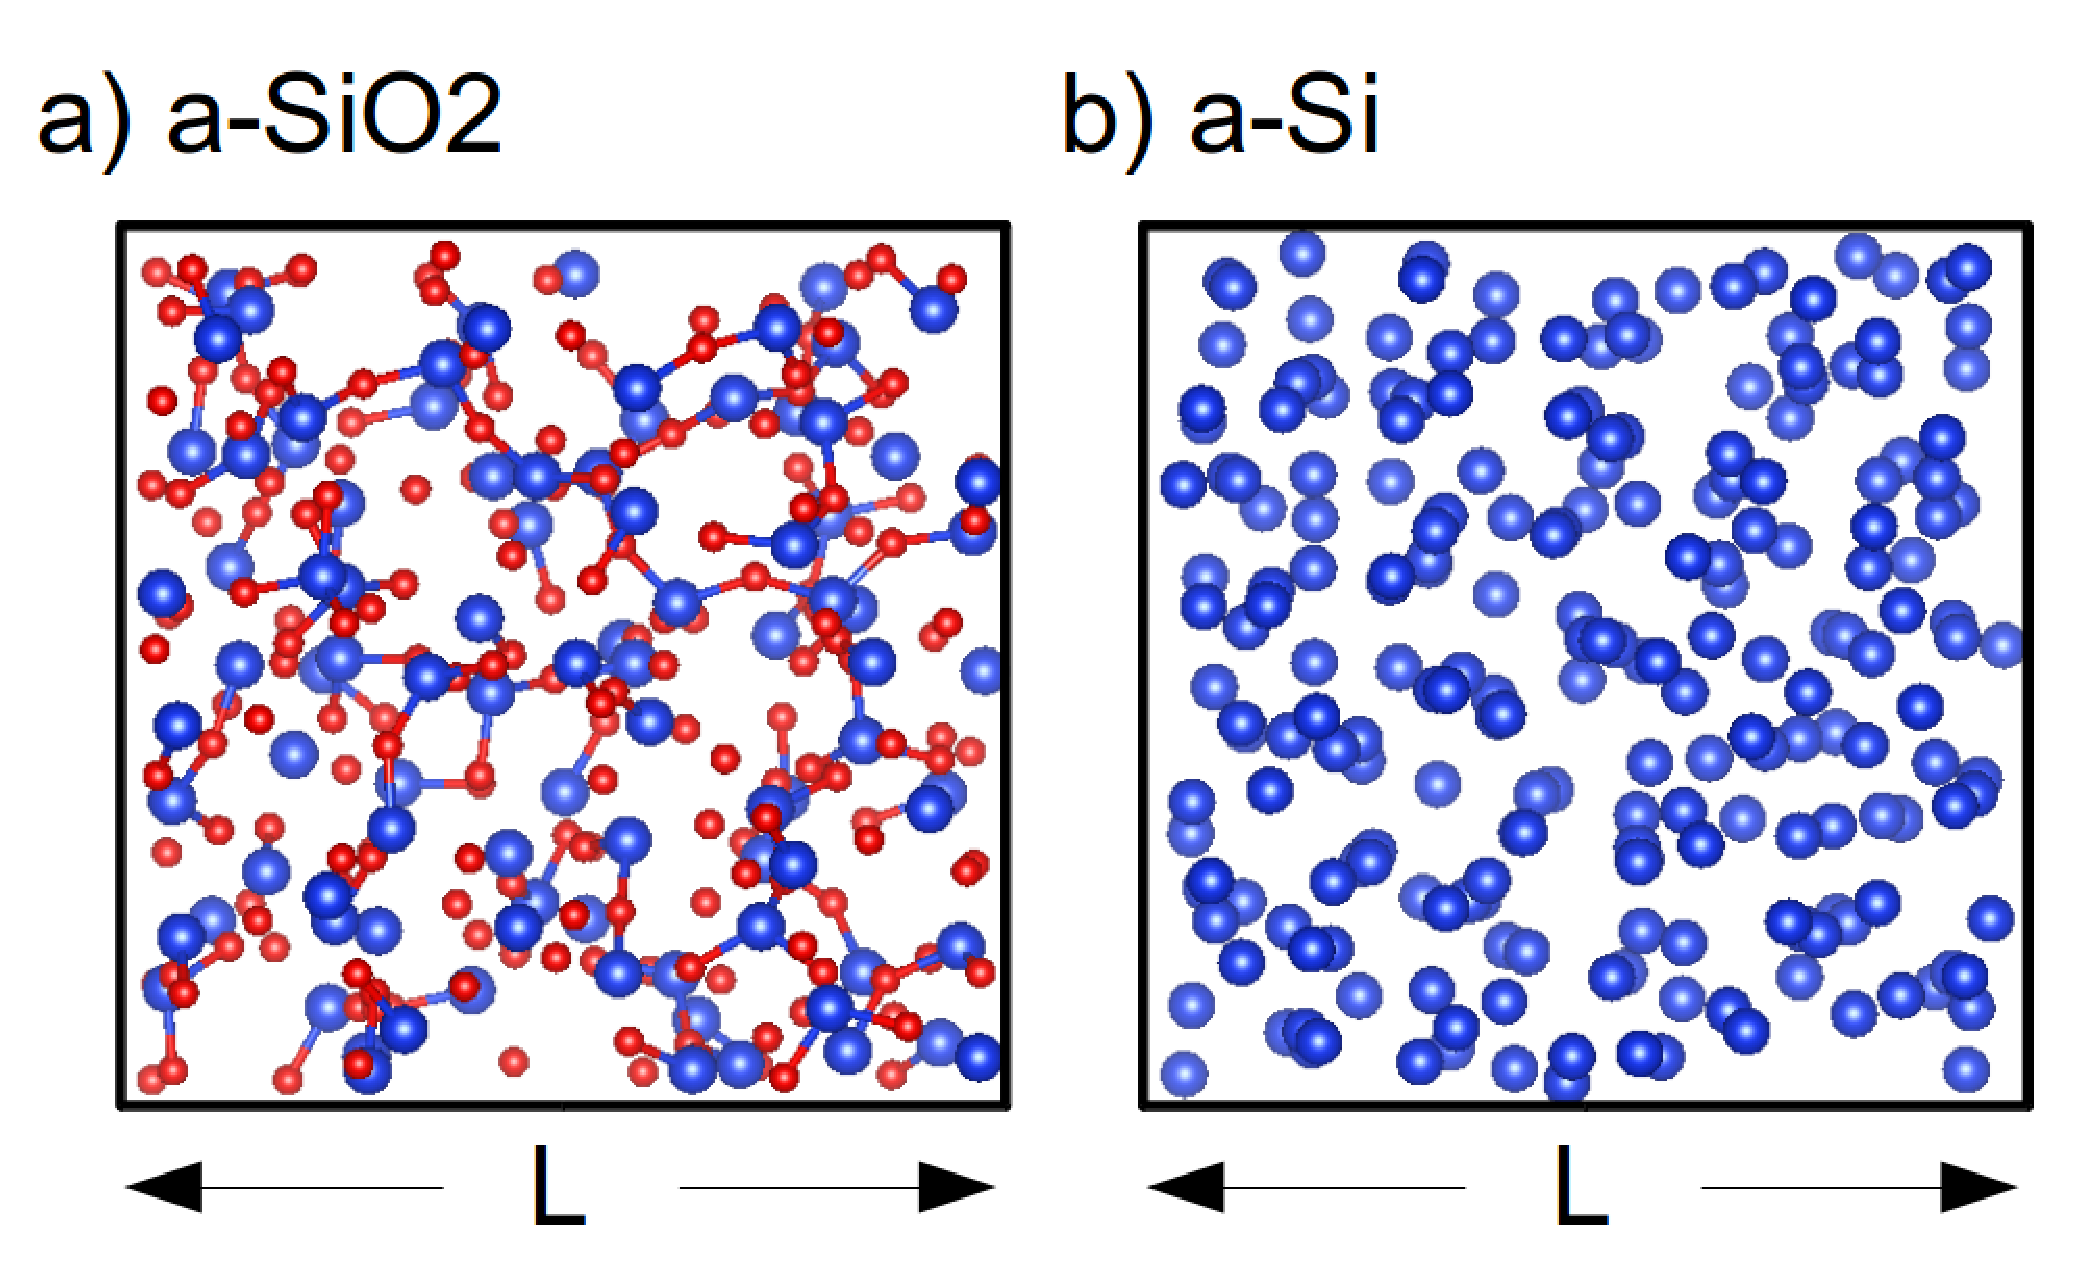
\includegraphics[scale=0.25]
{/home/jason/disorder/si/amor/init216_combined.eps}
\vspace*{-5mm}
\end{center}
\caption{\label{FIG:supercell} 
(a) a sample supercell of a-SiO2 with $N_a = 288$ and cell length 
$L=$ 1.597 nm. Samples up to size 
$N_a = 4,608 (36,864)$ and $L=4.026 (8.052)$ nm are used for the 
LD(MD)-based methods in Sections and . The samples were prepared using 
(b) a sample supercell of a-Si with $N_a = 216$ and cell length 
$L=$ 1.597 nm. Samples up to size 
$N_a = 4,096 (800,000)$ and $L=4.344 (24.81)$ nm are used for the 
LD(MD)-based methods in Sections and . The a-Si samples were prepared 
using a modified WWW algorithm (see Section ).
Both a-SiO2 and a-Si structures are visualized using the 
VESTA package.\cite{momma_vesta:_2008}
}
\end{figure}
%--------------------------------------------------------------------------

%--------------------------------------------------------------------------
\subsection{\label{S:Simulation}Simulation Details}
%--------------------------------------------------------------------------

Molecular dynamics (MD) simulations are performed using the disordered 
a-SiO$_2$ and a-Si supercells described in 
Section \ref{S:Sample}. 
The MD simulations were performed using LAMMPS\cite{plimpton_fast_1995}  
with time steps of dt = 0.00905 (0.0005) ps for a-SiO$_2$(a-Si). 
Ten MD simulations with different initial conditions were run and 
the predictions from these simulations were ensemble averaged. 
All MD simulations are first equilibrated in a NVT (con-
stant number of atoms, volume, and temperature) ensemble for $10^6$ 
time steps. Data are then collected from simulations
in the NVE (constant number of atoms, volume, and total
energy) ensemble 
for $2^21$ time steps and the atomic trajectories sampled 
ever $2^8$ time steps. 

The Green-Kubo (GK) method is used to predict the thermal 
conductivity $k_{GK}$ (see Section ) from MD simulations of the 
largest supercells of a-SiO2 and a-Si (see Section ). The 
$k_{GK}$ is predicted by window averaging the integral of the heat current 
autocorrelation function (HCACF).(cite) For a-SiO$_2$ and s-Si, a 
interval of the the HCACF integral can be found which is constant 
within the statistical noise.(cite) Similar $k_{GK}$ (within 
the errors) are predicted using the first avalanche method.(cite)  
For $N_a=4,608 (4,096)$, the trajectories from the MD simulations 
used for the GK method are also used with the NMD method to predict 
the vibrational mode lifetimes of a-SiO2(a-Si) (Section \ref{S:Life}). 

For the amorphous supercells studied,
the only allowed wave vector is the gamma-point (i.e., $\pmb{\kappa}=0$),  
where $\pmb{\kappa}$ is the wavevector and there are $3N_a$ polarization 
branches labeled by $\nu$. 
Calculation of the 
vibrational modes at the Gamma point (referred to as Gamma modes) 
require the eigenvalue solution 
of a dynamical matrix of size 
$(3N_a)^2$ that scales as $[(3N_a)^2]^3$, limiting the system 
sizes that can be considered to $N_a = 4,608(4,096)$ for 
a-SiO$_2$(a-Si). 
The eigenvalue solution is required to predict the vibrational 
density of states (DOS (see Section ), structure factors 
(see Section ), perform the NMD technique  
(see Section \ref{S:Life})  
and perform the AF calculations (see Section \ref{S:Diffusivities}). 
The frequencies and eigenvectors were computed using harmonic
lattice dynamics calculations and GULP.\cite{gale_general_2003} 
The calculation of the AF diffuson thermal diffusivities 
(Eq. \eqref{EQ:DAF}) 
is performed using GULP and a Lorentzian 
broadening of $14\delta\omega_{avg}$($5\delta\omega_{avg}$) for 
a-SiO$^2$(a-Si), where $\delta\omega_{avg}$ is the average mode 
frequency spacing ($\delta\omega_{avg} = ()$ for a-SiO2(a-Si)).
(cite) For a-Si the broadening is within $20\%$ of that used 
in Ref \citenum{feldman_numerical_1999}(CHECK). 
Varying the broadening around these values does not 
change the resulting thermal conductivity $k_{AF}$ significantly 
(see Section ). 

%--------------------------------------------------------------------------
\section{\label{S:Vibrational}Vibrational Properties}
%--------------------------------------------------------------------------

%--------------------------------------------------------------------------
\subsection{\label{S:DOS}Density of States}
%--------------------------------------------------------------------------

In this section, we examine the frequencies and density of states (DOS)  
for the Gamma modes for our models of a-SiO$_2$ and a-Si. 
The vibrational DOS is computed by 
\begin{equation}\label{EQ:DOS}
DOS(\omega) = \sum_i \delta(\omega_i - \omega),
\end{equation}
where a unit step function is used to broaden 
$\delta(\omega_i - \omega)$.(cite)  
The DOS for a-SiO$_2$ and a-Si are plotted in Fig. \ref{FIG:DOS} 
using a broadening of $10\delta\omega_{avg}$ and $100\delta\omega_{avg}$.  
Because of the finite model size, the low-frequency modes are sparse and 
the DOS can depend on the broadening.
\cite{feldman_numerical_1999} We use a broadening which is large enough 
to obtain good statistics but also small enough to extend 
to low frequencies.   

The DOS for a-Si is similar to the 
DOS of crystalline silicon,
\cite{williams_numerical_1985,donadio_atomistic_2009} particularly 
at low-frequency, and with pronounced features at mid-range and high 
frequencies, as in disordered lattices.
\cite{larkin_predicting_2013,beltukov_ioffe-regel_2013} The DOS for 
a-SiO$_2$ is essentially constant over most of the frequency-range, 
with a gap at the higher frequencies due to the presence of 
the oxygen atoms.(cite)   
There is a clear scaling of $DOS \propto \omega^{-2}$ for both 
a-Si and a-SiO$_2$ at the lowest frequencies. 
The onset of this scaling occurs at a higher frequency 
for a-Si than a-SiO$_2$. The DOS scaling at the lowest 
frequencies for a-SiO2 and a-Si suggest that the modes may be 
propagating (phonon-like),  
which is investigated in the following sections. 

% The observation that the acoustic modes are located on
% top of a flat background for intermediate values of q has re-
% cently been found by G ̈
% otze and Mayr as an essential
% result in their analytic calculation of the spectra within
% mode-coupling theory.
% \cite{gotze_evolution_2000}
% 
% The DOS predicted for a-SiO2 is similar to previous 
% models\cite{taraskin_phonons_1997} as well as 
% experimentally measured DOS.(cite)
% 
% The DOS predicted for jammed systems are similarly dominated by 
% the transverse sound speed,\cite{vitelli_heat_2010} 
% while results for disordered lattices demonstrate 
% \cite{beltukov_ioffe-regel_2013,larkin_predicting_2013}

%--------------------------------------------------------------------------
\begin{figure}
\begin{center}
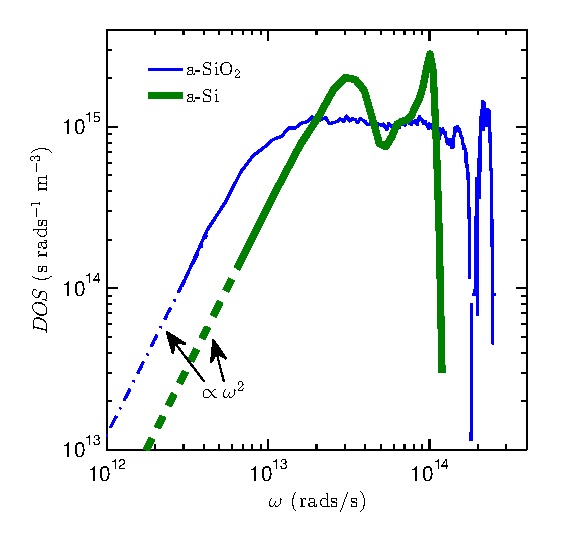
\includegraphics[scale=1.0]
{/home/jason/disorder/si/amor/m_af_si_normand_4096_DOS_3.eps}
\vspace*{-5mm}
\end{center}
\caption{\label{FIG:DOS} Vibrational DOS predicted for our 
models of a-SiO2 and a-Si using Eq. \eqref{EQ:DOS}. Both models 
show a scaling at low frequency $DOS(\omega)\propto\omega^{-2}$, 
which is predicted by the Debye approximation 
(Eq. \eqref{EQ:DOS_debye}) using the transverse sound speeds 
predicted using various methods (Table \ref{T:vs}). At high frequency, 
the DOS of a-SiO2 shows a plateau and then a sharp feature corresponding 
to a gap in the vibrational spectrum due to the Si and O bonds.(cite) 
For a-Si, there are two sharp peaks, which show as small peaks in the 
predictions of the vibrational mode lifetimes (Fig. \ref{FIG:Lifetimes}) 
and mode diffusivities (Fig. \ref{FIG:diffusivities}).}
\end{figure}
%--------------------------------------------------------------------------
%\clearpage
%\vspace{50mm}

%--------------------------------------------------------------------------
\subsection{\label{S:Structure}Structure Factor}
%--------------------------------------------------------------------------

Calculating the structure factors of the supercell Gamma   
modes is a method to test for their propagating plane-wave 
character at a particular wave vector and 
polarization. 
\cite{allen_diffusons_1999,feldman_numerical_1999} 
The structure factor has been used to predict effective 
dispersion of amorphous materials 
experimentally(cite more)\cite{green_density_2011} 
and 
numerically (cite more).
\cite{feldman_numerical_1999,volz_molecular-dynamics_2000} 
The structure factor at a wave vector 
$\pmb{\kappa}$ is defined as\cite{allen_diffusons_1999} 
\begin{equation}\label{EQ:SLT}
S^{L,T}\kw = 
\sum_{\nu} E^{L,T}\kv
\delta (\omega-\omega\kgv),
\end{equation}
where the summation is over the Gamma modes, $E^{T}$ refers 
to the transverse polarization and is defined as
\begin{equation}\label{EQ:EL}
E^L\kv = 
\left|
\sum_{b} 
\hat{\pmb{\kappa}} \cdot e\kgvba 
\EXP{i\pmb{\kappa}\cdot\pmb{r}_0\ab{l=0}{b}} 
\right|^2
\end{equation}
and $E^{L}$ refers to the longitudinal polarization and is defined as
\begin{equation}\label{EQ:ET}
E^T\kv = 
\left|
\sum_{b} 
\hat{\pmb{\kappa}} \times e\kgvba 
\EXP{i\pmb{\kappa}\cdot\pmb{r}_0\ab{l=0}{b}} 
\right|^2.
\end{equation}
In Eqs. \eqref{EQ:EL} and \eqref{EQ:ET}, the $b$ summations are 
over the atoms in the disordered supercell, 
$\pmb{r}_0\ab{l=0}{b}$ refers to the equilibrium atomic position of 
atom $b$, $l$ labels the unit cells 
($l=0$ for the supercell), 
$\alpha$ labels the Cartesian coordinates, and 
$\hat{\pmb{\kappa}}$ is a unit vector.  
The vibrational ``mode shape'' is contained in the 
$3N_a$ components of its eigenvector, $e\kgvba$.

The structure factors $S^{L,T}\knw$ are plotted in Fig. 
\ref{FIG:disp} for 
a-SiO$_2$ and a-Si (left and right panels) for wavevectors along the 
[100] direction of the 
supercells. Because of isotropy, the direction is not important 
and the wavenumber can be considered instead of wavevector. 
The wavenumbers are normalized by a length scale $a$ so that 
$\kappa = 1$ corresponds to $2\pi/a$. The length scale 
$a = $ 4.8(5.43) $\AA$ for a-SiO$_2$(a-Si), which is based 
on the lattice constants of c-SiO2(c-Si).(cite)

Frequencies $\omega_0(\kappa)$ and linewidths $\Gamma(\kappa)$ are 
predicted by fitting each structure 
factor peak $S^{L,T}\knw$ to a Lorentzian function
\begin{equation}\label{EQ:Lorentzian_SLT}
\begin{split}
S^{L,T}\knw = 
\frac{C_0(\pmb{\kappa})}{[\omega_0(\pmb{\kappa})-\omega]^2+\Gamma^2(\pmb{\kappa})},
\end{split}
\end{equation}
where $C_0(\nu)$ is a constant related to the DOS.
\cite{beltukov_ioffe-regel_2013} A dispersion relation is identified by 
plotting $\omega_0(\kappa)$ in the middle panel of Fig.\ref{FIG:disp}, 
where the error bars 
indicate the linewidths $\Gamma(\kappa)$. 

For a-Si, the peaks are reasonably Lorentzian for all wavenumbers considered.
\cite{feldman_calculations_2002} 
For a-SiO2, the peaks are well-approximated as Lorentzian only at the 
smallest wavenumbers. For 
large wavenumber, the structure factors peaks are much less than an order 
of magnitude larger than the background, and the widths are on the order 
of the frequency range considered in Fig. \ref{FIG:disp}.(cite) For 
large wavenumber the structrue factor takes on the form of the vibrational 
DOS. 

Fig 4 shows the dispersion extracted by locating the peaks in 
the structure factor for a-SiO2 and a-Si. For a-Si, the dispersion is 
nearly linear at small $\kappa$ with slight concave-down dispersion at 
high $\kappa$.(cite) For a-SiO2, the dispersion is concave-down for 
the smallest wavenumbers considered, transitioning to a strong 
concave-up dispersion at intermediate wavenumber. 
For intermediate $\kappa$, the longitudinal dispersion for a-SiO$_2$ 
is better-described by the so-called 
''dispersion law for diffusons``, where $\omega \propto \kappa^2$.
\cite{beltukov_ioffe-regel_2013} This large concave-up dispersion has been 
observed in various amorphous models\cite{feldman_calculations_2002} 
including of a-SiO2.\cite{ruzicka_evidence_2004} 
The dispersion predited by the structure factors show that a-Si 
has a near-linear, crystal-like dispersion while the dispersion 
for a-SiO2 is more diffuson-like,(cite) at least over the range of 
wavenumber and frequencies considered here.  At lower frequencies 
($< 100$ GHz)(cite), experimental measurements of a-SiO2 show a 
linear dispersion. 

%--------------------------------------------------------------------------
\subsection{\label{S:Structure}Group Velocity}
%--------------------------------------------------------------------------

The DOS and structure factors predicted in Sections and are now used to 
predict the group velocity of modes at the lowest-frequencies for 
a-SiO2 and a-Si. In the low-frequency, long-wavelength limit the 
mode group velocities are the sound speed.(cite) 
By fitting the DOS 
from Fig. \ref{FIG:DOS} to Eq. \eqref{EQ:DOS_debye}, 
a sound speed is predicted $v_{s,DOS}$ and 
reported in Table \ref{T:vs}. Because the DOS is a mixture of 
transverse and logitudinal modes only a single sound speed is predicted. 
Both logitudinal and transverse sound speeds can be predicted from 
the structure factor.(cite) 
Sound speeds are estimated from the structure factor peaks by finite 
differencing,\begin{equation}\label{EQ:vs_dwdk}
v_{s} = \frac{ \delta \omega_0(\kappa)}{\delta \kappa},
\end{equation}
and are shown in Table using the lowest frequency peaks 
from Fig. \ref{FIG:disp}. 
The transverse and longitudinal sound speeds of a material can 
also be predicted from the material's bulk ($G$) and 
shear ($K$) moduli.(cite) The transverse sound speed is given by(cite)  
\begin{equation}\label{EQ:vs_T_elas}
v_{s,T} = \frac{G}{\rho}^{1/2},
\end{equation}
and the longitudinal by
\begin{equation}\label{EQ:vs_L_elas}
v_{s,L} = \frac{4G + 3K}{3\rho}^{1/2}.
\end{equation}
We use the bulk and shear moduli defined in terms of the elastic 
constants according to the Voight convention.(cite) 
The sound speeds calculated from the 
elastic constants are reported in Table . 
The sound speeds predicted for a-Si in Table are in good agreement 
with those found in a previous study using a similar 
model.\cite{feldman_thermal_1993,feldman_numerical_1999} 
Comment about a-SiO2 sound speeds with expt and modeling.(cite)

It is clear that the DOS of 
our models for a-Si and a-SiO$_2$ are characterized by using the 
transverse sound speeds, rather than an averaging of the transverse 
and longitudinal which is commonly used,(cite)  
\begin{equation}\label{EQ:vs_avg}
v_{s} = \frac{2}{3}v_{s,L} + \frac{1}{3}v_{s,T}. 
\end{equation} 
The values of the transverse sound speeds obtained from the 
elastic modulii are somewhat larger than the structure factors, 
an indication of the concave-down dispersion seen at low 
$wavenumber$, particularly for a-SiO2 (Fig. ).
(cite) For a-SiO2, the concave-down dispersion
also affects the low-frequency DOS, where the predicted sound speed 
$v_{s,DOS}$ is less than that predicted from the structure factor 
and the elastic constants (Table ). The concave-down dispersion 
is less pronounced for a-Si, where the sound speeds predicted 
by all three methods are within five percent of each other. 

Under the Debye model (Eq. ), the $\emph{smaller}$ transverse sound speed 
makes the $\emph{larger}$ contribution to the DOS, scaling as the sound 
speed cubed. For a-Si, 
the contribution from longitudinal modes to the Debye DOS is nearly 
an order of magnitude less than the transverse modes for a given 
frequency interval. For a-SiO$_2$, the longitudinal and transverse 
sound speeds are closer, but the concave-down dispersion 
is stronger than a-Si (Fig. ).(cite experimental DOS) 
The intensity of the structure factors  
are directly proportional to the DOS.(cite)
The intensity for the dynamic structure factor of transverse 
polarizations has been found to be four to five\cite{taraskin_phonons_1997} 
and 6-8\cite{horbach_high_2001} times larger than longitudinal 
polarizations for models 
of a-SiO2, which supports our finding that the DOS is dominated 
by transverse modes. 
The transverse sound speed predicted by the DOS $v_{s,DOS}$ is used for both 
a-SiO$_2$ and a-Si throughout the rest of this work and is discussed 
in Section .

For a disordered solid, 
except for the transverse and longitudinal sound speeds, there is not an 
accepted method to predict the group velocity of each  
vibrational mode. 
While the structure factor gives the frequency spectrum needed to 
construct a propagating state with pure wavevector $\pmb{\kappa}$, 
the mode spectrum $E^{T,L}\kv$ (Eqs. and ) predicts the plane-wave 
character of each mode. As shown previously, it is not possible 
in general 
to assign a unique wavevector to individual modes, even at low frequency,
\cite{biswas_vibrational_1988,feldman_thermal_1993,silbert_normal_2009} 
which makes predicting individual mode group velocities challenging. 
Attempts have been made to predict individual mode group velocities,
\cite{cahill_lattice_1988,duda_reducing_2011,donadio_atomistic_2009,
he_heat_2011,he_thermal_2011,hori_phonon_2013} 
but 
it is not clear that these methods are consistent with the predictions 
made by the structure factor, in this work and in others.(cite) 
In the Cahill-Pohl (CP) model, for example, the group velocity of 
all disordered modes is the sound speed, $v_s$, which is also assumed  
for the HS model Eq. \eqref{EQ:M:k_AF,HS}.
\cite{cahill_lattice_1988} This assumption is not generally valid  
for any material.\cite{feldman_numerical_1999,duda_reducing_2011,
donadio_atomistic_2009,he_heat_2011,he_thermal_2011,larkin_predicting_2013}
To treat this problem, the thermal diffusivities of 
vibrational modes in a-SiO2 and a-Si 
are predicted and compared in Section  to test the assumption of the 
mode group velocities at all frequencies. 

% Experimentally determined values
% Freeman gives 4100 m/s for a-SiO$_2$\cite{freeman_thermal_1986}
% 3,700 5,100 from \cite{pohl_low-temperature_2002}
% for a-Si 3,800-4,800\cite{pohl_low-temperature_2002}
% Experimentally measured values of sound speed for a-Si are 4,160
% \cite{senn_physics_1979} and 
% 4,290 m/s\cite{vacher_attenuation_1980}.
% \cite{feldman_elastic_1991} 
% For chemical vapor depositioned a-Si thin films, the transverse 
% sound speed is markedly increased $v_{s,T} = 4,740$ m/s.
% \cite{liu_high_2009} 

%--------------------------------------------------------------------------
\begin{figure}
\begin{center}
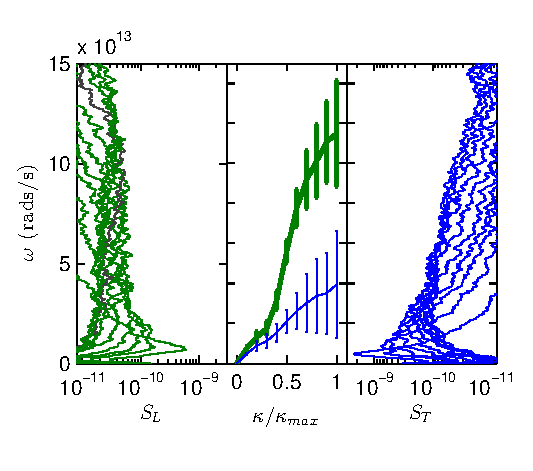
\includegraphics[scale=1.0]
{/home/jason/disorder/si/amor/m_af_si_normand_4096_disp_sio2_2.eps}
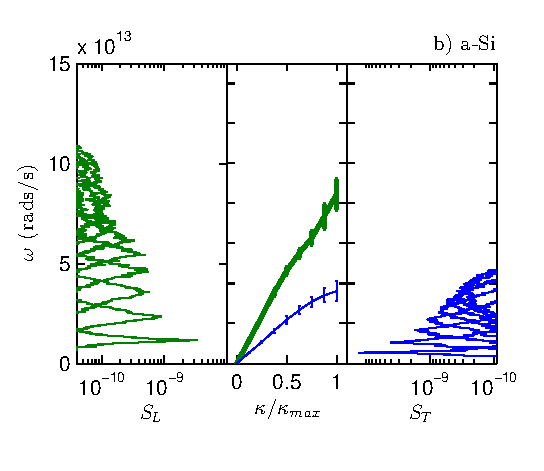
\includegraphics[scale=1.0]
{/home/jason/disorder/si/amor/m_af_si_normand_4096_disp_si.eps}
\end{center}
\caption{\label{FIG:disp} Longitudinal (left panel) and transverse 
(right panel) structure factors (Eq. \eqref{EQ:SLT}) for a-SiO2 (top 
plot) and a-Si (bottom plot). Sound speeds are estimated by finite 
differencing (Eq. \eqref{EQ:vs_dwdk}) of the lowest frequency peaks and 
are reported in Table \ref{T:vs}. The dispersion for a-SiO2 is only 
linear for the lowest frequency, smallest wavenumbers. The dispersion 
for a-Si is linear over a wider range of wavenumber. Lifetimes are 
predicted from the widths of the structure factor peaks 
(Eq. \eqref{EQ:Lorentzian_SLT}) and are 
plotted in Fig. \ref{FIG:Lifetimes}. }
\end{figure}
%--------------------------------------------------------------------------

%--------------------------------------------------------------------------
\begin{center}
%\begingroup
\squeezetable
\begin{table}
\caption{\label{T:vs}
Estimated from the elastic constants, the pre-annealed group velocities are 
$v_{s,T,} = 3,670$ , $v_{s,L,elas} = 7,840$ for a-Si and
$v_{s,T,elas} = 2,541$ , $v_{s,L,elas} = 4,761 $ for a-SiO2 
(see Section \ref{S:Structure}).
}
\begin{ruledtabular}
\begin{tabular}{llllll}
\hline
method~~~~~~~\vline Eqs. \eqref{EQ:vs_T_elas}, \eqref{EQ:vs_L_elas} ~~~\vline Eqs. \eqref{EQ:SLT}, \eqref{EQ:vs_dwdk} ~~~~~~~~ \vline DOS Eq. \eqref{EQ:DOS_debye}  \\
\hline
a-SiO$_2$  \\
\hline
transverse~~~~\vline 3,161~~~~~~~~~~~~~~~ \vline 2,732~~~~~~~~~~~~~~~~~~~~~~ \vline 2,528  \\
\hline
longitudinal~\,\vline 5,100~~~~~~~~~~~~~~~ \vline 4,779~~~~~~~~~~~~~~~~~~~~~~ \vline   \\
\hline
a-Si  \\
\hline
transverse~~~~\vline 3,886~~~~~~~~~~~~~~~ \vline 3,699~~~~~~~~~~~~~~~~~~~~~~ \vline 3,615  \\
\hline
longitudinal~\,\vline 8,271~~~~~~~~~~~~~~~ \vline 8,047~~~~~~~~~~~~~~~~~~~~~~ \vline   \\
\end{tabular}
\end{ruledtabular}
\end{table}
%\endgroup
\end{center}
%--------------------------------------------------------------------------

%\clearpage
%\vspace{50mm}

%--------------------------------------------------------------------------
\subsection{\label{S:Life}Mode Lifetimes}
%--------------------------------------------------------------------------

We now predict the lifetimes of all vibrational modes in our 
models of a-SiO2 and a-Si using the MD simulation-based normal mode 
decomposition (NMD) method.
\cite{ladd_lattice_1986,mcgaughey_quantitative_2004,
turney_predicting_2009-1,larkin_comparison_2012} 
The NMD-predicted lifetimes will be 
compared with the timescales extracted from the structure 
factor linewidths, $\tau_{SF} = 1/2\Gamma(\kappa)$ 
(Section , (Eq. \eqref{EQ:Lorentzian_SLT})). 
The NMD method can predict vibrational lifetimes which are affected by 
the disorder in the supercell.
\cite{he_heat_2011,he_thermal_2011,he_morphology_2011,he_lattice_2013,
larkin_predicting_2013}

In NMD, the 
atomic trajectories from MD simulations are first mapped onto the vibrational 
mode coordinate time derivative,
\cite{dove_introduction_1993}
\begin{equation}\label{EQ:qdot}
\begin{split}
\dot{q}\kgvt{}{}{}=&\SUM{0}{}\sqrt{\frac{m_b}{N}}\dot{u}_{\alpha}
\lbt e^*\kgvba\EXP{i(\pmb{0}\cdot\mathbf{r}_0\ab{l}{0}}.
\end{split}
\end{equation}
Here, $m_b$ is the mass of the $b_{th}$ atom in the supercell, 
$u_{\alpha}$ is the $\alpha$-component of the atomic displacement 
from equilibrium, $\dot{u}_{\alpha}$ is the $\alpha$-component 
of the atomic velocity, and $t$ is time. Because the supecells 
of a-SiO2 and a-Si are disordered, the NMD method is performed at 
the wavevector $\pmb{\kappa} = \pmb{0}$. 
The spectral energy of each vibrational mode, $\Phi\kvt$, is calculated 
from 
\begin{equation}\label{A:E:Phi_NMD}
\begin{split}
\Phi(\nu,\omega) = 
\lim_{\tau_0\rightarrow\infty}\frac{1}{2\tau_0}
\left|\frac{1}{\sqrt{2\pi}}\int_{0}^{\tau_0}\dot{q}\kgvt
\exp(-i\omega t)dt\right|^2.
\end{split}
\end{equation}
We choose the frequency domain representation of the normal mode 
energy because it is less sensitive to any meta-stability 
of the amorphous structure.(footnote) 
(footnote)In an amorphous material, there are many potential energy 
configurations 
(atomic positions) which are nearly equivalent in energy.  At a sufficient 
temperature, the meta-stable configurations cause the equilibrium 
atomic positions to vary in time.  This can effect on the prediction of 
the vibrational mode 
lifetimes when using the normal 
mode decomposition method. In the time domain, the average normal 
mode potential and kinetic energy must be calculated and subtracted 
from the normal mode energy autocorrelation function.(cite) 
If the average 
energy is not specified correctly, unphysically large or small mode 
lifetimes can be predicted.(cite) 

The vibrational mode frequency and lifetime is predicted by fitting each mode's 
spectral energy $\Phi(\nu,\omega)$ to a Lorentzian function
\begin{equation}\label{EQ:Lorentzian_NMD}
\begin{split}
\Phi(\nu,\omega) = 
\frac{C_0(\nu)}{[\omega_0(\nu)-\omega]^2+\Gamma^2(\nu)},
\end{split}
\end{equation}
where the constant $C_0(\nu)$ is related to the average energy of 
each mode and the linewidth $\Gamma(\nu)$ and is valid when 
$\Gamma(\nu) < \omega_0(\nu)$.\cite{larkin_comparison_2012} 
The mode lifetime is given by(cite) 
\begin{equation}\label{EQ:NMD_life}
\begin{split}
\tau(\nu) = \frac{1}{2\Gamma(\nu)}
\end{split}
\end{equation}

The NMD-predicted lifetimes are plotted in Fig. \ref{FIG:Lifetimes} 
for a-SiO2 and a-Si. 
For a-SiO2, the mode lifetimes are generally larger than 
the IR limit $\tau = 2\pi/\omega$,(cite) and follow 
this limit at low frequency. There is no clear evidence for a
quadratic scaling $\tau\propto\omega^{-2}$, which 
corresponds to a quadratic scaling of the diffusivity at low 
frequency where the group velocity is constant 
(Eq. \eqref{EQ:Dtau}). 
At high frequency the mode lifetimes are roughly constant 
without definite scaling. There is a peak near 
2 $10^{14}$ rads$/$s which corresponds to a peak in the DOS 
(see Fig. \ref{FIG:DOS}).  The lifetimes predicted from the 
structure factor fall below the NMD-predicted lifetimes 
and the IR limit. This is because the structure factor for 
a-SiO2 is evaluated for large enough wavenumber that the 
peaks are not well-approximated as Lorentzian.(cite) Fitting 
the peaks we find the linewidth (inverse lifetime) 
to be on the order of the frequency range considered in 
Fig. \ref{FIG:disp}. 
Models(cite) and theoretical(cite) predictions show that the 
structure factor begins to take on the form of the DOS 
for large enough wavenumber,
\cite{martin-mayor_dynamical_2001,baldi_thermal_2008} and the 
linewidths (timescales) are not meaningful. For a-SiO2 the NMD and 
structure factor-predicted lifetimes indicate that the 
low-frequency modes 
in our model are not well-characterized as propagating.(cite)  

For a-Si, 
The mode lifetimes show a clear scaling at low frequency 
$\tau\propto\omega^{-2}$. The lifetimes plateau at higher frequencies,
over a wider range of frequencies than a-SiO2, with two peaks 
corresponding to peaks in the DOS (Fig. \ref{FIG:DOS}). The plateau of 
lifetimes at high frequencies has been 
reported for disordered lattices
\cite{sheng_heat_1991,larkin_predicting_2013} and 
other models of a-Si.\cite{he_heat_2011} 
The transition from the quadratic low-frequency scaling to 
the plateau region occurs near 
$10^{14}$ rads$/$s, which corresponds to where the DOS peaks in Fig. 
\ref{FIG:DOS}. 
Similar behavior was observed for models of disordered lattices.
\cite{larkin_predicting_2013} The lifetimes predicted by the 
structure factor are in good agreement with those predicted by NMD 
at low frequencies. Similar agreement has been reported in other 
models of topologically disordered materials.
\cite{mazzacurati_low-frequency_1996} 
The longitudinal and transverse polarizations 
outline the scatter in the NMD-predicted lifetimes. While the DOS 
at low frequency is 
dominated by transverse modes, the NMD and 
structure factor-predicted lifetimes indicate there 
is some mixture of longitudinal and transverse-like modes.(cite) 

The NMD-predicted lifetimes in this work are similar in magnitude to 
those predicted for previous models of a-Si.
\cite{bickham_calculation_1998,bickham_numerical_1999} 
Fabian and Allen find lifetimes on the order of picoseconds for a-Si
\cite{fabian_anharmonic_1996} and para-crystalline silicon.
\cite{fabian_numerical_2003} 
A previous study of Tersoff a-Si predicted vibrational lifetimes on 
the order of 100 ps, about ten times the values reported here and in 
other studies.(cite) It is unclear what the source of this 
discrepancy is, although the analysis in Ref \citenum{he_thermal_2011} 
the NMD method in the time domain. Using the Tersoff potential on the 
WWW a-Si models in this work we find...
Predicted lifetimes are also similar for 
samples created using a melt-quench technique 
(see Section \ref{S:Sample:Si}).

%--------------------------------------------------------------------------
\begin{figure}
\begin{center}
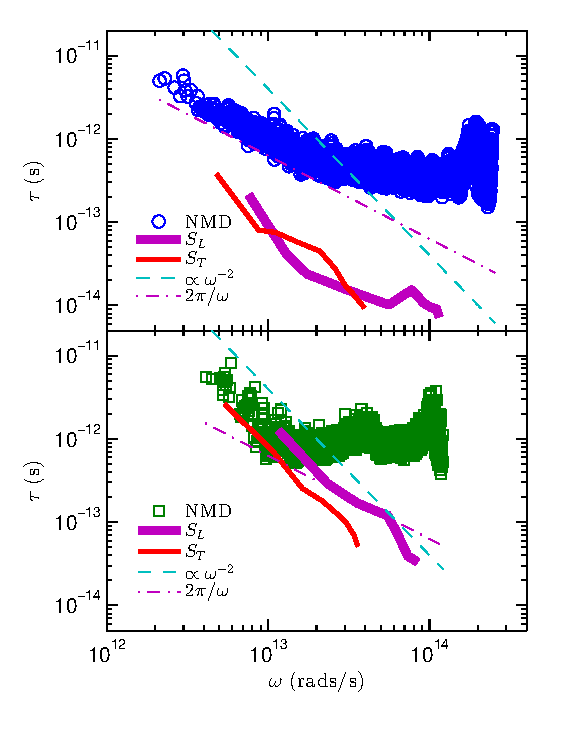
\includegraphics[scale=1.0]
{/home/jason/disorder/si/amor/m_af_si_normand_4096_tau_2.eps}
\vspace*{-5mm}
\end{center}
\caption{\label{FIG:Lifetimes} vibrational mode lifetimes predicted by 
NMD (Eq. \eqref{EQ:NMD_life}) and the structure factors 
(Eq. \eqref{EQ:Lorentzian_SLT}) for a-SiO2 (top plot) and 
a-Si (bottom plot).  The IR limit is a lower limit for the 
NMD-predicted lifetimes, while the lifetimes from the structure factors 
fall below this limit, particularly for a-SiO2. The structure factor 
lifetimes generally follow a scaling $\tau\propto\omega^{-2}$ for both 
systems, while the NMD-predicted lifetimes show a plateau before 
crossing the IR limit. }
\end{figure}
%--------------------------------------------------------------------------

%--------------------------------------------------------------------
%\begin{figure}
%\begin{center}
%\includegraphics[scale=1.0]
%{/home/jason/disorder/si/amor/m_si_amor_life_he_compare.eps}
%\vspace*{-5mm}
%\end{center}
%\caption{\label{FIG:phonon_diff} film thickness dependant thermal 
%conductivity of a-Si from experiment.}
%\end{figure}
%--------------------------------------------------------------------------

%--------------------------------------------------------------------------
\subsection{\label{S:Diffusivities}Diffusivities}
%--------------------------------------------------------------------------

Using the sound speeds predicted 
from the DOS $v_{s,DOS}$ (Table ), the NMD-predicted lifetimes are 
used to predict the mode diffusivities with Eq. \eqref{EQ:Dtau} 
and are shown in Fig. for a-SiO2 and a-Si. 
The sound speed is most appropriate  
for the lowest-frequecy modes (see Section ). To compare with the 
NMD predictions, the AF theory is also used to predict the mode 
diffusivities (see Section ) which are shown in Fig. . 

For a-SiO2 at the lowest frequencies, the 
diffusivities scale roughly as Eq. with $n=2$.  However this 
scaling is not definitive for the diffusvities predicted by either 
method, particularly for the NMD predictions, which 
is apparent from the scaling of the NMD-predicted lifetimes 
in Fig. . To identify the transition from propagating 
to non-propagating modes, we use $\omega_{cut} = 4.55$ rad$/$s 
for Eq. , 
the same as that used in Ref \citenum{baldi_thermal_2008} since 
there is no clear indication of this tranistion from Fig. . 
This choice is discussed in Section . The constant 
$B=$ is Eq. 
is fit to the AF-predicted diffusivities for 
$\omega \le \omega_{cut}$.

For a-Si at low frequencies there is a clear scaling of the 
diffusivities Eq. with $n=2$.  
The NMD-predicted diffusivities show much less 
scatter than those predicted by the AF theory, which is due to 
the finite-size system and the broadening which is required to evaluate 
Eq. \eqref{EQ:DAF}.\cite{feldman_thermal_1993} By using a much larger 
broadening ($~100\delta\omega_{avg}$) the scatter in the AF-predicted 
diffusivities at low frequency can be smoothed, but at the cost of 
decreasing the diffusivities at intermediate and high frequencies. 
It is possible that a frequency-dependent broadening may be necessary 
for a-Si and the AF theory,(cite)  
but determining this dependence is not clear nor necessary for 
interpreting the results in this work.  

For a-Si, we choose $\omega_{cut}$ and $B$ so that Eq. is equal 
to the AF-predicted diffusivity at $\omega=\omega_{cut}$. This choice 
allows Eq. to pass reasonably well through both the AF and NMD-predicted 
diffusivities.  The value of $\omega_{cut}$ and $B$ are comparable to 
those used in Ref. .  For a-Si we also consider a separate scaling 
for Eq. with $n=4$ which is discussed in Section . Because this 
scaling is not clear from the data in Fig. we use 
$\omega_{cut} = $ 1.52 $10^13$ rads$/$s  
from Refs. \ref{feldman_numerical_1999} and \ref{cahill_lower_1994} 
and choose $B$ so that Eq. is equal to the AF-predicted 
diffusivity at $\omega_{cut}$. We discuss these choices in Section . 

For a-SiO2, the mode diffusivities predicted by NMD and AF agree 
well over the entire frequency range. At high frequencies the 
diffusivities do not vary much, except for a 
peak for the NMD predictions near 2 $10^{14}$ rads/s which 
corresponds to the same peak in lifetimes (Fig. ). For 
the AF predictions, the mode diffusivities near 
2 $10^{14}$ rads/s and at the highest frequencies 
show a sharp decrease, which is an indication 
that these modes are localized.(cite) 

Both a-SiO$_2$ and a-Si have a region at higher frequencies where the 
AF-predicted mode diffusivities are relatively constant. This behavior 
has been reported for a number of model disordered systems such as 
disordered lattices
\cite{sheng_heat_1991,beltukov_ioffe-regel_2013,larkin_predicting_2013}, 
amorphous solids,\cite{he_thermal_2011} 
and jammed systems.\cite{xu_energy_2009,vitelli_heat_2010}  
For a-Si the NMD- and AF-predicted diffusivities diverge 
near 1 $10^{13}$ rads$/$s, while the NMD-predicted lifetimes 
are relatively constant above this frequency.  This implies 
that the velocity scale for diffusons,
\begin{equation}\label{EQ:vAF}
\begin{split}
v_{AF}(\omega) = \left(3\frac{D_{AF,i}(\omega)}{\tau(\omega)}\right)^{1/2},
\end{split}
\end{equation}
is a function of frequency. At low frequencies, $v_{AF}$ 
reaches as high as $v_{s,DOS}$ and decreases to about $(1/3) v_{s,DOS}$ 
at higher frequencies. This variation of $v_{AF}(\omega)$ is similar 
to the variation of the group velocity which can be estimated from 
the dispersion relation found in Fig. . For a-SiO2, $v_{AF}$ is near 
$v_{s,DOS}$ over the whole frequency range, which is the assumption 
made for the high-scatter limit Eq. .

(WORK)

The dependence of $v_{AF}$ with frequency for a-Si is similar to 
that found for 
simple crystalline systems, where negative dispersion typically 
causes a decrease of group velocity with increasing frequency (or 
wavevector).(cite) Negative dispersion has been predicted by many 
models of both a-SiO2 and a-Si,\cite{ruocco_relaxation_2000} 
as have experimental measurement of 
dispersion relations.(cite) The effective group velocities 
which have been predicted using dispersion relations near zero 
wavevector for large supercells of amorphous\cite{he_thermal_2011,he_heat_2011} 
and disordered lattices\cite{hori_phonon_2013} would appear to 
be underestimates 
compared with the effective velocities $v_{AF}$ predicted in this work, 
where $v_{AF}$ is within a factor of three of $v_s$ for all but the 
highest frequency, localized modes.(cite) Our predictions for 
$v_{AF}$ also support the notion of a minimum thermal diffusivity 
on the order of $D_{HS}$ for all vibrational modes except   
those which are localized (the so-called ''locons'').(cite) 

While diffusons are non-propagating modes whose MFPs are not 
well-defined, a diffuson MFP can be defined as
\begin{equation}\label{EQ:LambdaAF}
\begin{split}
\Lambda_{AF}(\omega) = (3D_{AF,i}(\omega)\tau(\omega))^{1/2},
\end{split}
\end{equation}
where $\tau(\omega)$ are the NMD-predicted lifetimes. Using this 
definition, $\Lambda_{AF}(\omega)$ is found to vary 
for a-SiO2 and a-Si between 
the supercell size $L$ and the lattice constant $a$ 
(see Section ) for modes with $\omega > \omega_{cut}$. 
Similar MFPs have been estimated for a-Si in 
previous studies.\cite{feldman_thermal_1993,feldman_numerical_1999} 
This is in contrast to the MFPs estimated in Ref \citenum{he_heat_2011}
which were found to be up to approximately $70 L$. The reason 
for this discrepancy is some combination of the predicted lifetimes 
and the method with which the mode group velocities were estimated.
\cite{he_heat_2011}

% To predict $k_{vib}$ we choose $\omega_{cut}$, 
% the constant $B$ for the diffusivity scaling, and the sound speed 
% $v_{s}$. For both a-SiO2 and a-Si, we use the sound speeds predicted 
% by a fit to the low-frequency DOS (Fig. \ref{FIG:DOS}). 
% For a-Si, the constant $B$ for the quadratic scaling is chosen such 
% that $D(\omega) = D_{AF,i}$ for $\omega_i=1.16$ rad$/$s. This value 
% of $\omega_{cut}$ is somewhat smaller than that used in Ref and . 
% The constant $B$ we find is somewhat larger than that found in 
% Ref. and . We choose this $\omega$ because of the reasonable agreement 
% between the AF-predicted $D_{AF}$ and NMD-predicted $D_{NMD}$ in this 
% frequency region, shown in Fig. \ref{FIG:diffusivities}. 
% 
% For a-Si a quadratic scaling is also 
% considered using $\omega_{cut}$ from the study by . As there is no clear 
% evidence of a quartic scaling of diffusivity, we choose the constant 
% $B$ to pass visibly through both $D_{AF}$ and $D_{NMD}$ in 
% Fig. \ref{FIG:diffusivities} because there is no clear procedure 
% to perform a fit. Our choice of $B=9.0 10^{46}$ m$^@$/s (rads$/$s)^4 
% for the quartic scaling is nearly the same as a fit\cite{cahill_lower_1994} 
% to the diffusivities in Ref \citenum{feldman_thermal_1993}, 
% $B=1.23 10^{47}$ m$^@$/s (rads$/$s)^4. 
% When using the quartic diffusivity scaling $D(\omega)\propto\omega^{-4}$, 
% the thermal conductivity is divergent as the frequency goes to zero.
% (cite) The thermal conductivity can be made finite using a boundary 
% scattering models,(cite) such as the simple one considered in 
% Section \ref{S:Bulk}. 
% While a fit to our model is not possible for the quartic scaling, 
% it has been used to explain previous experimental measurements of 
% a-Si thin films.(cite)
% 
% Baldi et al used a $\omega_{cut}=$ $4.55$ rads$/$s, which is a 
% reasonable 
% cut-off for our model of a-Si.\cite{baldi_thermal_2008} 
% Baldi et al find that the contribution $k_{ph}~0.1$ W/m-K, which is 
% the same as the contribution $k_{ph}$ predicted in this work for 
% a-SiO2. This contribution 
% $k_{ph}$ is smaller than the error bars in the predictions of $k_{vib}$ 
% and $k_{GK}$ shown in Figs. and .  
% 
% The quadratic scaling of mode diffusivities at low frequencies 
% for a-Si 
% is responsible for the system size dependent thermal conductivity 
% predicted by the GK method $k_{GK}$. 
% While our model is best described by 
% quadratic scaling, we are modeling bulk a-Si. 

% Based on the NMD-predicted diffusivities, the modes at low frequency are 
% dominated by transverse modes. However, given the scatter in the 
% NMD-predicted lifetimes, there is some mixture of 
% transverse and longitudinal 
% modes at low frequency.  Treating these two branches separately 
% is not necessary since similar results are obtained by assuming a single 
% branch scaling $D(\omega)=B\omega^{-2}$ which is fit to coincide with the 
% peak in diffusivity $D_{AF}$ at $\omega_{cut} = $ 11.6 E 12 rads/s. This 
% choice of $\omega_{cut}$ is close to that used by 
% FAB ($\omega_{cut}$ = 9.65 E 12 rads/s),\cite{feldman_thermal_1993} 
% and is somewhat smaller than 
% that used by FKAW\cite{feldman_numerical_1999} 
% and Cahill et al.\cite{cahill_thermal_1994} 
% ($\omega_{cut}$ = 15.2 E 12 rads/s). 


% It was shown that the diffusivity $D_{AF}(\omega) \propto DOS(\omega)$ 
% at low frequency when the modes are spatially uncorrelated and the 
% overlap between them is small and independent of the frequency.
% \cite{vitelli_heat_2010,xu_energy_2009} This result helps to explain 
% the plateau of diffusivity for both a-SiO2 and a-Si at higher 
% frequencies. The features in $D_{AF,i}$ for both a-SiO2 and a-Si can 
% be explained by peaks in the DOS at these frequencies. 

%--------------------------------------------------------------------------
\begin{figure}
\begin{center}
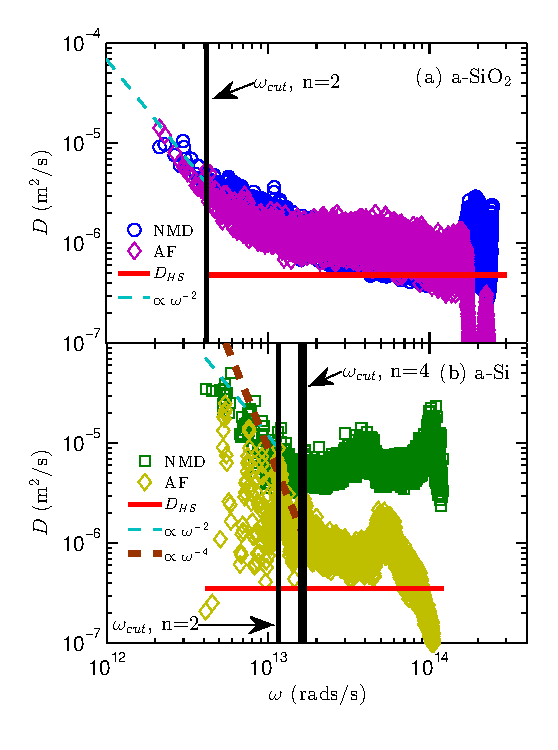
\includegraphics[scale=1.0]
{/home/jason/disorder/si/amor/m_af_si_normand_4096_D_4.eps}
\vspace*{-5mm}
\end{center}
\caption{\label{FIG:diffusivities} vibrational mode diffusivities 
predicted from NMD (using Eqs. \eqref{EQ:Dtau} and \eqref{EQ:NMD_life} 
with the sound speed $v_{s,DOS}$ 
from Table \ref{T:vs}) and AF theory (Eq. \eqref{EQ:DAF}). 
Also shown are the 
extrapolations Eqs. \eqref{EQ:Dw2} and \eqref{EQ:Dw4}, which are used 
with Eq. \eqref{EQ:kph} to predict the thermal conductivity accumulations 
in Fig. \ref{FIG:accum}, and the high-scatter limit Eq. \eqref{EQ:D_HS}. 
}
\end{figure}
%--------------------------------------------------------------------------

%--------------------------------------------------------------------------
% \begin{figure}
% \begin{center}
% \includegraphics[scale=1.0]
% {/home/jason/disorder/si/amor/m_af_si_normand_4096_vAF.eps}
% \vspace*{-5mm}
% \end{center}
% \caption{\label{FIG:Lifetimes} .}
% \end{figure}
%--------------------------------------------------------------------------

%\clearpage
%\vspace{50mm}

% %--------------------------------------------------------------------------
% \begin{figure}
% \begin{center}
% \includegraphics[scale=1.0]
% {/home/jason/disorder/si/amor/m_af_si_normand_4096_Lambda_3.eps}
% \vspace*{-5mm}
% \end{center}
% \caption{\label{FIG:mfp} vibrational MFPs predicted from NMD using Eq. 
% \eqref{EQ:Lambda} and the sound speed predicted in Table \ref{T:vs}
% and from NMD and AF using Eq. \eqref{EQ:LambdaAF}. Good agreement 
% between the two methods is seen at low frequency, indicating that the 
% modes are propagating and Eqs. \eqref{EQ:Dtau} and \eqref{EQ:DLambda} 
% are valid. The majority of MFPs in the intermediate the high-frequency range 
% lie between the simulation box size $L$ and the bond distance $a$. The 
% inset compares the representative mode velocities Eq. \eqref{EQ:vAF} and 
% the sound speeds. For a-Si, $v_{AF}$ decreases with increasing frequency, 
% similar to the behavior of a monatomic crystal.(cite) The MFPs and 
% mode velocities only approach zero at the highest frequencies, which is 
% an indication that the modes are localized.}
% \end{figure}
% %--------------------------------------------------------------------------

%\clearpage
%\vspace{50mm}

%--------------------------------------------------------------------------
\section{\label{S:Conductivity}Thermal Conductivity}
%--------------------------------------------------------------------------

%--------------------------------------------------------------------------
\subsection{\label{S:Bulk}Bulk}
%--------------------------------------------------------------------------

To predict the bulk thermal conductivity for our models of a-SiO2 and 
a-Si, we use Eq. \eqref{EQ:kvib} 
and the GK method.(cite) The GK method for predicting 
thermal conductivity
is relatively inexpensive compared to the NMD and AF methods so  
large system sizes can be studied (see Section \ref{S:Sample:Si}).  
Similarly-large 
systems were studied in Ref. \citenum{he_heat_2011}. The details of the 
GK method are discussed in Section \ref{S:Simulation}. 

The GK-predicted thermal conductivity $k_{GK}$ is plotted in 
Fig. \ref{FIG:cond} for 
varying system sizes $L$. For a-SiO2, there is no apparent dependence 
of $k_{GK}$ on $L$ and $k_{GK}=2.1 \pm 0.15$ W/m-K. 
For a-Si, there is a clear dependence of $k_{GK}$ on 
$L$. Assuming the DOS has the form of Eq. \eqref{EQ:DOS_debye} 
and the diffusivity scaling 
is Eq. \eqref{EQ:Dw2} with $n=2$ 
for the low-frequency modes in the system, 
the thermal conductivity as a function of the system size 
takes the form
\begin{equation}\label{EQ:k0}
\frac{k(L)}{k_{bulk}} = 1 - \frac{c_0}{L},
\end{equation}
where $k_{bulk}$ is the extrapolated bulk thermal conductivity and $c_0$ 
is a constant.\cite{shiomi_thermal_2011,esfarjani_heat_2011} 
The extrapolation is performed using the three largest 
system sizes studied, including the tiled 800,000 atom sample (see 
Section \ref{S:Sample:Si}). 
We do not observe that tiling an a-Si model increases 
the thermal 
conductivity of a given system size above that predicted by Eq. , as 
was found in Ref \citenum{he_thermal_2011} using the MD-based 
direct method. This is likely due to the 
small (512 atom) model used to perform the tiling in that study, 
while we use a 100,000 atom model. 
The success of 
Eq. \eqref{EQ:k0} for the dependence of $k_{GK}$ on 
$L$ for our model of a-Si is in 
agreement with the scaling Eq. \eqref{EQ:Dw2} with $n=2$ 
(Fig. \ref{FIG:diffusivities} 
and the Debye-scaling of the DOS (Fig. \ref{FIG:DOS}). 
The extrapolated $k_{bulk} = 1.9 \pm 0.1$ W/m-K

To predict $k_{vib}$ (Eq. ) we use the input parameters 
$B$, $\omega_{cut}$, and the AF-predicted diffusivities 
$D_{AF}(\omega)$ obtained in Section . 
For a-SiO2, $k_{AF} = 1.92$ and $k_{pr} = 0.09$ W/m-K. 
Baldi et al find that the contribution $k_{ph}~0.1$ W/m-K, which is 
the same as the contribution $k_{ph}$ predicted in this work for 
a-SiO2. This contribution 
$k_{ph}$ is smaller than the error bars in the predictions of $k_{vib}$ 
and $k_{GK}$ shown in Figs. and .  


For a-Si with Eq. and $n=2$, 
$k_{AF} = 1.16$ and $k_{pr} = 0.62$ W/m-K. For Eq. and $n=4$, the 
diverging conductivity at low frequency is fixed by the 
use of a simple boundary scattering model based on the Matthiesen 
rule and the thin-film thickness $t_f$,\cite{sellan_cross-plane_2010} 
\begin{equation}\label{EQ:LambdaMatth}
\begin{split}
\frac{1}{\Lambda_{eff}} = \frac{1}{\Lambda_{bulk}} + 
\frac{2}{t_f}.
\end{split}
\end{equation}
Using 

$k_{pr} = 2.98$ W/m-K

Using the $n=2$ scaling and $t_f = 80,000$ nm does not change 
$k_{pr}$ within the precision reported. For $t_f = 50$ nm, 
$k_{pr} = 0.22$ for $n=4$ and $k_{pr} = 0.34$ for $n=2$. 






We predict for a-Si $k_{ph} = 0.62$ 
W$/$m-K. Similar values for $k_{ph}$ can be predicted by increasing 
$\omega_{cut}$ and decreasing $B$. 

The same $\omega_{cut}$ was used by Cahill et al. 
together with a Rayleigh scaling and a boundary scattering model to 
find $k_{ph} = 0.31$ W/m-K.\cite{cahill_thermal_1994} 

Comparing with previous MD simulations of a-Si, 
Lee found a value of around 1 W/m-K 
but with very small supercell sizes.\cite{lee_molecular-dynamics_1991}
He et al find for bulk a-Si $k_{vib} = 3$ W/m-K using the Tersoff 
potential and a linear extrapolation of the form Eq. using 
non-equillibrium molecular dynamics. In this study He at al find 
that $k_{pr} \approx k_{AF} \approx 1.5$ W/m-K.  Regner et al find 
a plateau in $k_{vib}$ for large broadband FDTR frequencies 
implying that $k_{AF} \approx 1$ W/m-K.(cite) 


Assuming a constant contribution  
$k_{AF} \approx 1$ W/m-K, experimental 
measurements and estimates show that the contribution from 
$k_{pr}$ is $~20\%$,


While the classic limit for the mode specific heat is 
an over-prediction for the high frequency modes in a-Si, 
the non-propagating contribution 
predicted by broadband FTDR matches the prediction from the AF 
diffuson theory. Adjusting the specific heats to include quantum 
statistical effects...

We can thus focus on the less understood low-frequency propagating contribution. 


For a diffusivity scaling Eq. with $n=4$ the thermal conductivity 
is divergent in the zero frequency limit. The s

















Phonon-like behavior 
can be identified for a-Si in this work and others, 
both experimentally
\cite{liu_high_2009,yang_anomalously_2010,minnich_thermal_2011,
regner_broadband_2013} 
and numerically.
\cite{feldman_thermal_1993,feldman_numerical_1999,
mcgaughey_thermal_2004,he_heat_2011} 
Including the phonon-like contribution $k_{ph}$ 
for a-Si is not qualitatively sensitive 
to the choice of model
\cite{feldman_thermal_1993,feldman_numerical_1999,liu_high_2009} 
or $\omega_{cut}$.
\cite{feldman_thermal_1993,feldman_numerical_1999,
donadio_atomistic_2009,liu_high_2009,yang_anomalously_2010}




% The relative contribution of $k_{ph}$ and $k_{AF}$ is also predicted to 
% be similar for silicon nanowires.\cite{donadio_atomistic_2009} 


%--------------------------------------------------------------------------
\begin{figure}
\begin{center}
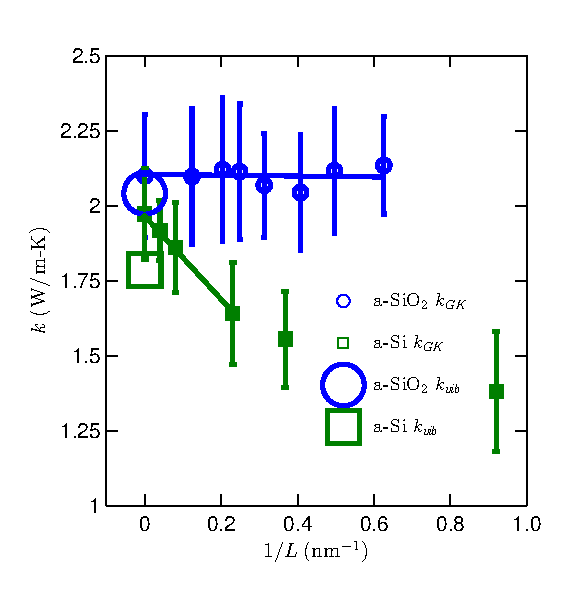
\includegraphics[scale=1.0]
{/home/jason/disorder/si/amor/m_af_si_normand_4096_gk_cond_2.eps}
\vspace*{-5mm}
\end{center}
\caption{\label{FIG:cond} Thermal conductivities of a-SiO$_2$ and 
a-Si prediced using the GK method. For a-SiO2, the thermal conductivity 
is size-independent, indicating there is no important contribution 
from phonons (Eq. \eqref{EQ:kph}). For a-Si, there is a clear size 
dependance, which is accounted for by using Eq. \eqref{EQ:kph} and 
an $\omega^{-2}$ extrapolation (Eq. \eqref{EQ:Dw2}, 
Fig. \ref{FIG:diffusivities}). }
\end{figure}
%--------------------------------------------------------------------------

%--------------------------------------------------------------------------
\subsection{\label{S:Accumulation}Accumulation Function}
%--------------------------------------------------------------------------

BEGINALAN

The thermal conductivity accumulation function,
\begin{equation}\label{EQ:matth}
k(\Lambda_{cut}) = \frac{1}{V}\int^{\Lambda_{cut}}_{0} 
kb D(\Lambda)DOS(\Lambda)    
+ 
\frac{1}{V}\sum_{\Lambda{\AF} < \Lambda_{cut}} kb v_{AF}\Lambda_{AF},
\end{equation}
is predicted using our models of bulk a-SiO2 and a-Si and shown in Fig. . 
For the phonon contribution $k_{ph}$, the mode diffusivities 
$(D(\omega)$ can be transformed $D(\Lambda) = D(\omega)/v_s$. 


The thermal conductivity accumulation functions for 
a-SiO2 and a-Si thin films are shown in Fig. . 
The thermal conductivity accumulation function for a-SiO2 saturates 
at a MFP of 10 nm, which is on the order of the finite size 
of our model (Section \ref{S:Sample}). 
This sharp accumulation at small MFPs is 
in good agreement with the prediction that $k_{AF}$ is the dominant 
contribution to $k_{vib}$. This result is also in accord 
with the penetration depth-independent thermal 
conductivity measurements using broadband FDTR.
\cite{regner_broadband_2013} Only the quadratic scaling is 
considered for a-SiO2, which is discussed later in 
Section \ref{S:Accumulation}. 

For a-Si, the thermal conductivity accumulation function shows that 
$k_{AF}$ saturates before 10 nm, which is also on the order of our  
finite model size. The propagating contribution $k_{ph}$ is predicted 
using both quadratic and quartic scaling for the 
mode diffusivities. As discussed in Section \ref{S:Conductivity}, 
the quadratic scaling 
is responsible for the system size dependent thermal conductivity 
predicted by the GK method ($k_{GK}$, see 
Section \ref{S:Conductivity}) and seems to be 
the correct scaling to describe the low-frequency modes for our model 
of bulk a-Si. Using the quadratic scaling, the thermal accumulation 
functions for our model of a-Si thin films passes reasonably well 
through many of the experimentally measured values.(cite) The quartic 
scaling also passes through many of the experimentally measured 
values reasonably well, particularly for film thicknesses 
larger than 10 $\mu$m.(cite) 

ENDALAN

%--------------------------------------------------------------------------
\begin{figure}
\begin{center}
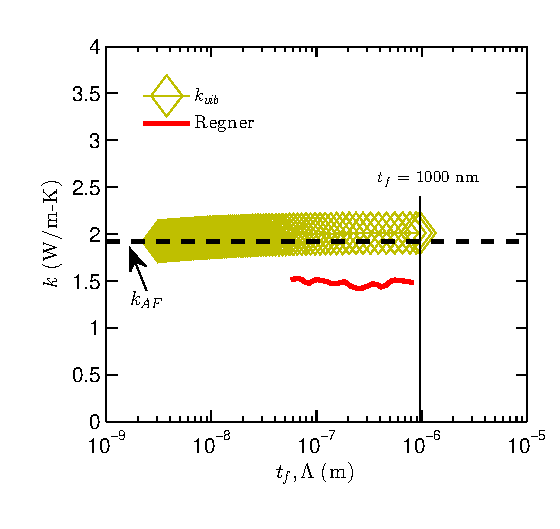
\includegraphics[scale=1.0]
{/home/jason/disorder/si/amor/m_af_si_normand_4096_kLamba_5_sio2.eps}
\vspace*{-5mm}
\end{center}
\caption{\label{FIG:accum} Thermal conductivity accumulations and thermal 
conductivities versus film thickness for a-SiO2 (top plot) and a-Si 
(bottom plot) from: (i) predictions from this work, (ii) recent broadband 
measurements of Regner et al, (iii) various experimental measurements 
for a wide-range of a-Si film thicknesses. While the thermal conductivity 
predictions for a-SiO2 and a-Si in this work seem to be well-characterized 
by Umklapp type scaling of the MFPs (Eq. \eqref{EQ:Dw2}), this scaling 
is not able to predict the dramatic increase of thermal conductivity 
with increasing film thickness from experimental measurements of a-Si thin 
films. }
\end{figure}
%--------------------------------------------------------------------------

%--------------------------------------------------------------------------
\begin{figure}
\begin{center}
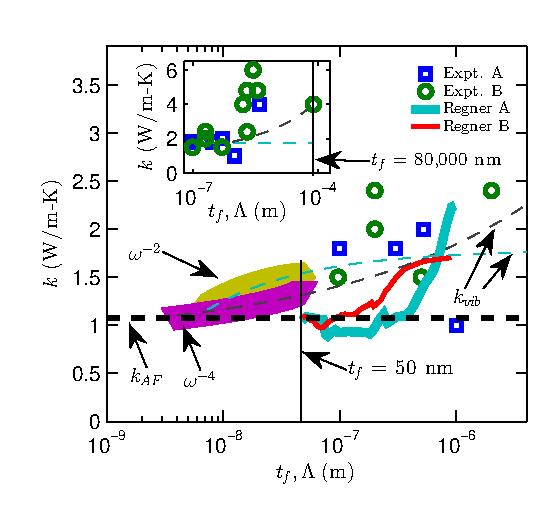
\includegraphics[scale=1.0]
{/home/jason/disorder/si/amor/m_af_si_normand_4096_kLamba_5_si.eps}
\vspace*{-5mm}
\end{center}
\caption{\label{FIG:accum} film thickness dependant thermal 
conductivity of a-Si from experiment.}
\end{figure}
%--------------------------------------------------------------------------

%\clearpage
%\vspace{50mm}

%--------------------------------------------------------------------------
\subsection{\label{S:Discussion}Discussion}
%--------------------------------------------------------------------------

BEGINALAN

Previous experimental studies of a-SiO2 have estimated negligible 
the contribution from 
low frequency ($\omega<\pi 10^12 rads/s$)\cite{love_estimate_1990} 
vibrational modes to be negligible. Using our model of a-SiO2, we also 
find the 
low-frequency propagating contribution to be negligible 
(Section \ref{S:Accumulation}). 
While experiments show there is are 
cross-over regions from quadratic to quartic scaling of the mode 
lifetimes in a-SiO2, the thermal conductivity of thin film a-SiO2 shows 
no significant dependence on the thickness.(cite) 
The cross-over 
region from quadratic to quartic, then back to quadratic 
observed in experiments for  
a-SiO2 occurs in the frequency range $4.6 10^9$ to 
$1.52 10^{10}$ rads$/$s,\cite{masciovecchio_evidence_2006} 
and $3.04 10^11$ to 
$1.52 10^{12}$ rads$/$s
\cite{baldi_emergence_2013}. 
While these frequency ranges are inaccessible by our finite-
size models, we estimate that the extrapolated $k_{ph}$ using a quartic 
scaling in this region to be... 

The transverse sound speed predicted for our model of 
a-SiO2 is about $85\%$ of that measured by experiment.\cite{liu_high_2009}  
While using a smaller transverse sound speed 
leads to an underprediction of the 
mode diffusivity scalings (Eq. \eqref{EQ:Dtau},
Fig. \ref{FIG:diffusivities} ), it leads to an 
overprediction of the DOS (Eq. \eqref{EQ:DOS_debye}). 
Overall this leads to an underprediction 
of the thermal conductivity because the DOS scales as 
$DOS(\omega)\propto 1/v^3_{s}$. We can regard the predictions from 
our models, with smaller transverse sound speeds, 
as an upper bound on $k_{ph}$ for a given diffusivity scaling 
$D(\omega) = B\omega^{-2}$. 
The critical parameter is the choice of $\omega_{cut}$.(cite) 
We pick 
$\omega_{cut}$ and the low frequency scaling $D(\omega) = B\omega^{-2}$ 
based on their ability to describe the low-frequency behavior 
of the vibrational modes in our finite-size models. The quadratic scaling 
$D(\omega) = B\omega^{-2}$ has been observed in separate numerical studies 
for models of a-SiO2(cite) and a-Si(cite). 

The bulk thermal conductivity predicted for our model of a-SiO2 overestimates 
that of experimental measurements.\cite{regner_broadband_2013} This can be 
attributed to either difference between experimental a-SiO2 and the 
potential model used in this work,(cite) the lack of anharmonic scattering 
included in the AF theory,\cite{feldman_thermal_1993} or the assumption 
of the classical-limit specific heat for all frequencies 
(Section \ref{S:Theory}). Qualitatively, 
our model confirms that propagating modes do not contribute significantly 
to the thermal conductivity of a-SiO2.
 
The classical-limit mode specific heat is a good approximation 
for the low-frequency propagating modes in a-SiO2 and a-Si, which are shown to 
fully activated by around 10 K.(cite) 
The classic limit for the mode specific heat is 
an over-prediction for the high frequency modes in a-SiO2 and a-Si at 300 K.(cite) 
However, the contribution $k_{AF}$ we predict in the classical limit 
for mode specific heat for a-Si is nearly the same as the 
the non-propagating contribution (plateau) predicted by broadband FTDR.(cite) 
Adjusting the specific heats to include quantum statistical effects...
Taking the diffuson contribution $k_{AF}$ to be a constant, which we predict 
to be $k_{AF} \approx 1$ W$/$m-K in agreement with other numerical 
studies(cite) and experiments(cite), 
we can thus focus on determining the less understood 
low-frequency propagating 
contribution $k_{ph}$. 

The scaling of the low-frequency lifetimes 
in a-Si is not clear from the experimental measurement. 
For a-Si thin films, varying preparation techniques suggest either 
quadratic(cite) or quartic(cite) scaling. 
While there is no clear consensus from various experiments, all predictions in this 
work demonstrate that  
the low-frequency modes in bulk a-Si follow a quadratic scaling 
of the mode lifetimes, which has been observed in previous models of 
a-Si(cite) and 
a-SiO2.(cite)
Amorphous silicon, however, can be
prepared only in thin films,(cite) where voids and other 
inhomogeneities are unavoidable\cite{li_effect_2011} and can influence the 
vibrational structure at low frequencies.
\cite{feldman_tight-binding_2004,liu_high_2009} 
A smooth transition between quadratic and quartic scaling can be 
achieved using a phenomenological model where a cross-over wavevector 
(or frequency) must be specified by experiment.
\cite{baldi_elastic_2011} While this cross-over can be identified 
experimentally for a-SiO2,\cite{masciovecchio_evidence_2006} 
experiments are limited for a-Si thin films.(cite) Our models 
are not large enough to investigate the relevant frequency range 
($< 1 10^{12}$ rads$/$s),(cite) so we considered both 
quadratic and quartic lifetime scalings when predicting 
the thermal conductivity accumulation functions in Fig. . 
Experimental measurements of the cross-over frequency (wavevector) and 
steepness parameter are needed from experiment to investigate the 
applicability of this phenomenological model further.(cite) 
The dependence 
of a-Si thin film thermal conductivity on thickness,(cite) 
preparation method,(cite) 
and hydrogen content(cite) make this particularly challenging. In fact, 
different experimental studies can be satisfactorily explained using 
quadratic(cite) or quartic(cite) scalings 
found that each was a satisfactory explanation for the results found.
(cite) 

A number of emerging experimental techniques are capable of 
studying the low-frequency propagating modes in disordered systems.
(cite) For amorphous materials, where the propagating contribution $k_{ph}$ 
is typically smaller than in the crystalline phase, broadband FDTR has demonstrated 
it can probe the relatively small effect of propagating modes at 300 K.  
However, the broadband FDTR studies thus far have been limited to one 
deposition technique and a relatively small range of film thicknesses 
($500$ nm $<t_{f}<$ 2000 nm).(cite) 
The nature of the low frequency scaling can be better elucidated using  
broadband FDTR on films prepared using 
varying deposition techniques,(cite) 
a wider-range of film thicknesses (1-100 $\mu$m)
(cite) 
and lower-range of temperatures ($~10-100$ K).(cite)
For a-Si, propagating low-frequency have been identified 
qualitatively by 
both experimental measurements(cite) and numerical modeling.(cite) 
It is thus interesting to consider thin films of a-SiGe alloys, which have been 
demonstrated to have reduced thermal conductivities compared to a-Si.
\cite{feldman_thermal_1993} It is not clear what vibrational lifetime scaling 
at low frequency would be observed in a simple topologically disordered alloy 
given there is no a consensus for even topologically disordered but chemically 
ordered systems.(cite) A combination of frequency-domain, time-domain, and 
variable-physical-heating size measurements would be helpful in investigating.
\cite{koh_frequency_2007,siemens_quasi-ballistic_2010,
minnich_thermal_2011,regner_broadband_2013}

ENDALAN

This supports the idea of Slack for a-SiO$_2$\cite{slack_thermal_1979}
While the thermal conductivity of a-SiO , the material is characterized by 
a constant similar for other amorphous
materials such as Lennard-Jones argon\cite{larkin_predicting_2013} 
and a model of a-GeTe.\cite{sosso_thermal_2012}

That the amorphous phase
of Si should have a lower GHz attenuation than many other
amorphous materials is not entirely surprising, as the 2002
review of low-temperature thermal conductivity and internal
friction by Pohl, Liu, and Thompson certainly indicates that
the fourfold coordinated materials tend to demonstrate weaker
anharmonicity.\cite{pohl_low-temperature_2002}

Theoretical predictions of acoustic attenuation in amor-
phous solids generally agree that at room temperature, a
quadratic frequency dependence is expected in the frequency
range of 10 GHz–1 THz and its origins are expected to be
the anharmonicity of the interatomic bonds.

Theory from Schirmacher et al. predicted 
an w4 scaling below a system dependent onset frequency.
\cite{schirmacher_thermal_2006,schirmacher_acoustic_2007}



%--------------------------------------------------------------------------
\section{\label{S:Lifetimes}Summary}
%--------------------------------------------------------------------------

BEGINALAN

In this work we investigated the contributions of propagating $k_{ph}$ and 
non-propagating $k_{AF}$ modes to the total vibrational 
thermal conductivity $k_{vib}$ of two glasses, a-SiO2 and a-Si. 
For a-SiO2, the contribution from propagating modes $k_{ph}$ is shown to 
be negligible compared to $k_{vib}$. This is confirmed by various 
experimental measurements, including a broadband FDTR study which 
probed the vibrational MFPs or a-SiO2. The thermal conductivity 
accumulation function for our model of a-SiO2 saturates near a MFP of 
10 nm, in agreement with the results of Regner et al. who show no 
systematic variation of the thermal conductivity on $L_p$,
\cite{regner_broadband_2013} and in agreement with experiments on 
a-SiO2 thin films which show no systematic variation with film 
thickness $t_f$.(cite) 

Our model of bulk a-Si has a thermal conductivity $k_{vib}$ with 
significant contribution from $k_{ph}$, where the low-frequency 
propagating modes are best described by a quadratic scaling of the 
mode lifetimes. 
The thermal conductivity accumulation predicted for our model of bulk 
a-Si with a simple boundary scattering model show reasonable agreement 
with some of the experimentally predicted thermal conductivities 
using varying film thicknesses and deposition techniques (Fig. ).(cite) 
However, using a quartic scaling with our model also gives 
a satisfactory agreement with other experimental measurements (Fig. ).(cite) 
These large discrepancies between measured 
thermal conductivity of various a-Si thin films calls for the need of 
further experimentation. Broadband techniques,(cite) which have demonstrated 
the ability to probe a wide-range of vibrational mode 
frequencies and MFPs, can help elucidate.(cite)

ENDALAN

%--------------------------------------------------------------------------
% \begin{center}
% %\begingroup
% %\squeezetable
% \begin{table}
% \caption{\label{T:cond_table}Thermal conductivity predictions using the 
% VC-NMD, VC-ALD, and GK methods. For LJ argon alloys, the bulk extrapolation 
% is used for all three methods.  For SW silicon alloys, only VC-ALD and GK 
% can be used to extrapolate a bulk thermal conductivity 
% (see Section \ref{S:Thermal Conductivity}). For VC-NMD and GK, the 
% uncertainties 
% are estimated by omitting independent simulations from 
% the ensemble averaging (see Section \ref{S:Calculation}). For VC-ALD, 
% the uncertainties are estimated by omitting extrapolation points used for 
% Eq. \eqref{EQ:k0}.}
% \begin{ruledtabular}
% \begin{tabular}{llllll}
% $c$  ~~~~\vline GK ~~~~~~~~~~~ \vline VC-NMD~~~~\, \vline VC-ALD~~~~~\, \vline VC-NMD$^*$~~~ \vline VC-ALD$^*$ ~~\: \vline  \\
% \hline
% LJ  \\
% \hline
% 0.00 \vline 3.3 $\pm$ 0.1 ~~~\, \vline 3.3 $\pm$ 0.1 ~~ \,\, \vline 3.4 $\pm$ 0.1 ~~~\,\,\, \vline ~~~~~~~~~~~~~~\;~\,\, \vline~~~~~~~~~~~~~\:\:\,\, ~ \vline \\
% 0.05 \vline 0.80 $\pm$ 0.07 \, \vline 0.76 $\pm$ 0.07 ~ \vline 0.45 $\pm$ 0.02 ~\, \vline 0.80 $\pm$ 0.1 \,  ~ \vline 0.52 $\pm$ 0.05  ~ \vline  \\
% \end{tabular}
% \end{ruledtabular}
% \end{table}
% %\endgroup
% \end{center}
%--------------------------------------------------------------------------

% %--------------------------------------------------------------------------
% \begin{figure}
% \begin{center}
% \includegraphics[scale=0.6]
% {/home/jason/disorder/matlab/galli_si_k_tf.eps}
% \vspace*{-5mm}
% \end{center}
% \caption{\label{FIG:phonon_diff} film thickness dependant thermal 
% conductivity of a-Si from experiment.}
% \end{figure}
% %--------------------------------------------------------------------------

\clearpage
\bibliographystyle{apsrev}
\bibliography{/home/jason/Dropbox/ntpl-paper/ntpl-060313}
\end{document}
% 